
\chapter{Análisis del sistema.}
\label{cap:capitulo_3}

En este capítulo vamos a detallar el funcionamiento todos los elementos analizados y utilizados para la elaboración del proyecto.

\section{Órgano de la Parroquia de la Encarnación}

El instrumento instalado en la Parroquia de la Encarnación de Santa Fe es en realidad un doble órgano artesanal construido en dos fases: En 1775 se instaló el primer órgano, de estilo barroco, obra del organero Pedro Ghys. Posteriormente, a principios de la década de 1830, el francés Guillermo D'Enoyer lo amplía añadiendo un órgano romántico, con un segundo teclado y nuevos sonidos, pero todo el mecanismo es independiente del primer instrumento.

\smallskip

\begin{figure}[H]
	\noindent \begin{centering}
		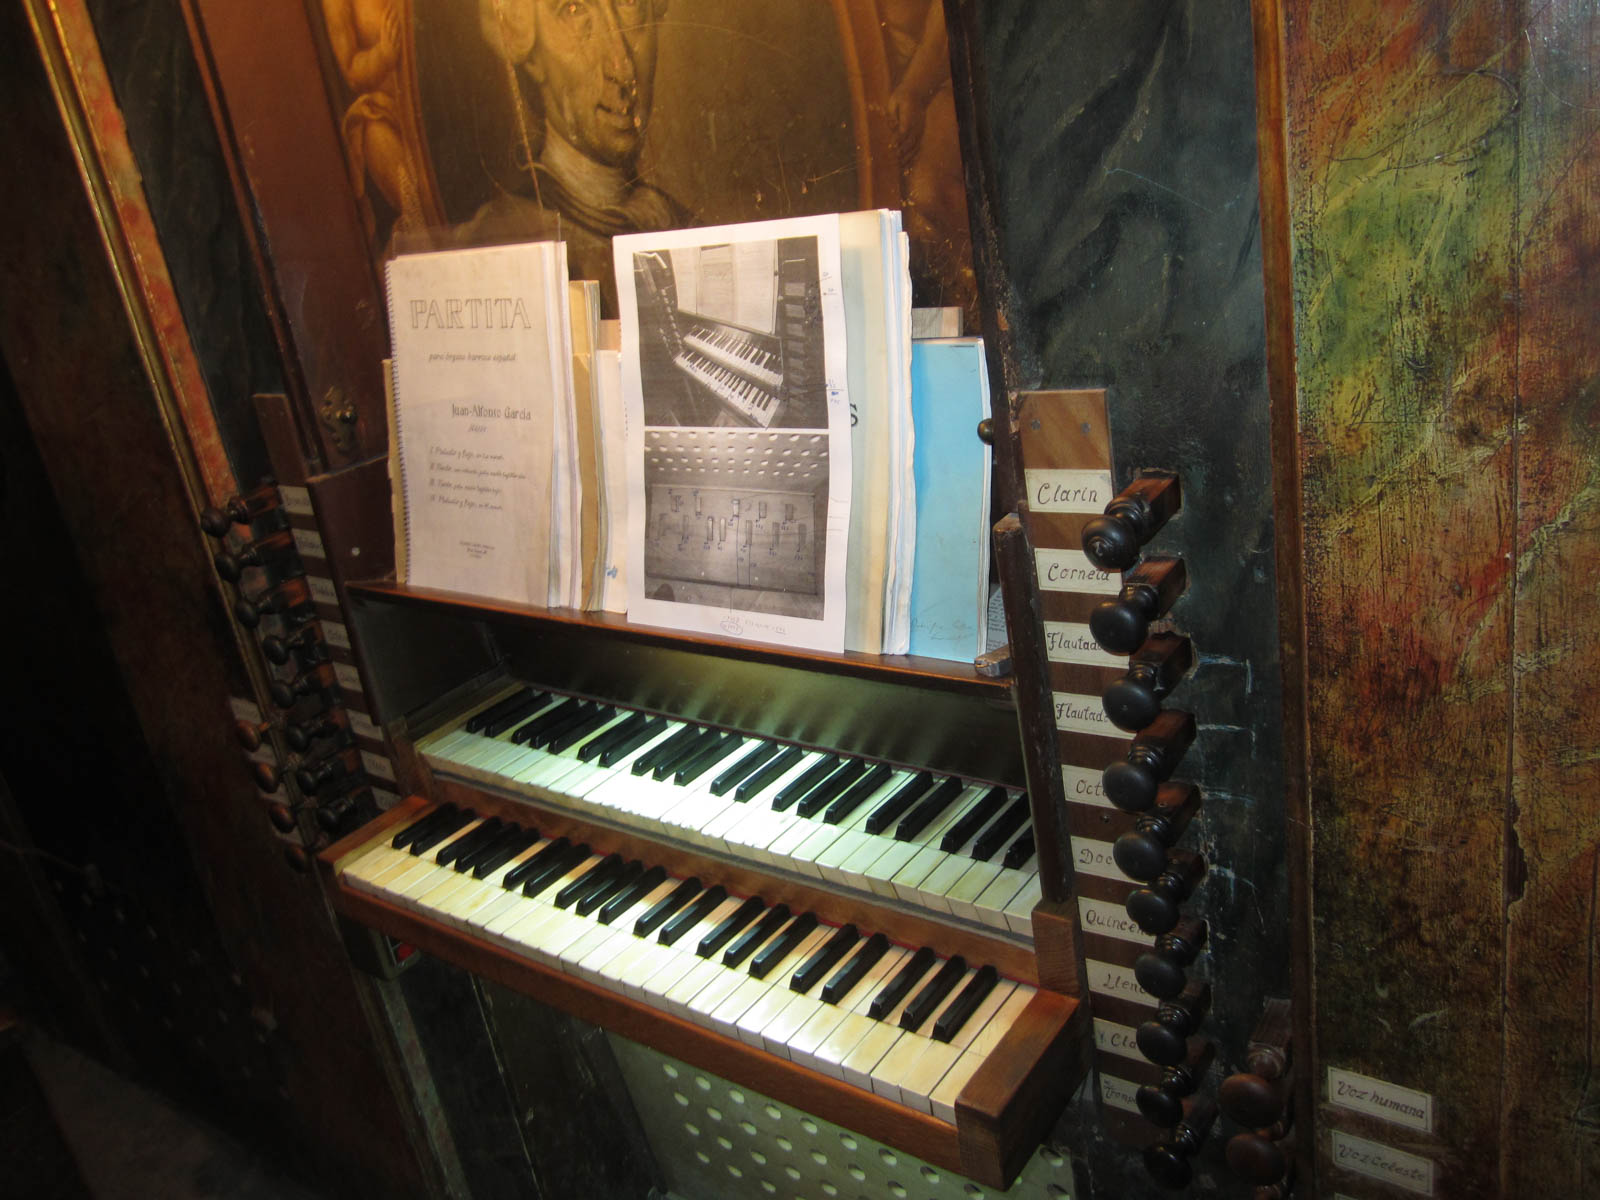
\includegraphics[width=\linewidth*3/4]{capitulo3/consola}
		\par\end{centering}
	\smallskip
	\caption{\label{fig:consola} Consola del órgano.}
\end{figure} 

\smallskip

Para funcionar, el órgano se alimenta de aire. Antiguamente se utilizaba un fuelle gigante, situado en la antesala, que llevaba el aire a una cámara de almacenamiento, para proporcionar un flujo de entrada constante. Esto requería que hubiese alguien follando mientras el organista tocaba. Hoy día el fuelle ha sido sustituído por una bomba eléctrica.

\smallskip

\begin{figure}[H]
	\noindent \begin{centering}
		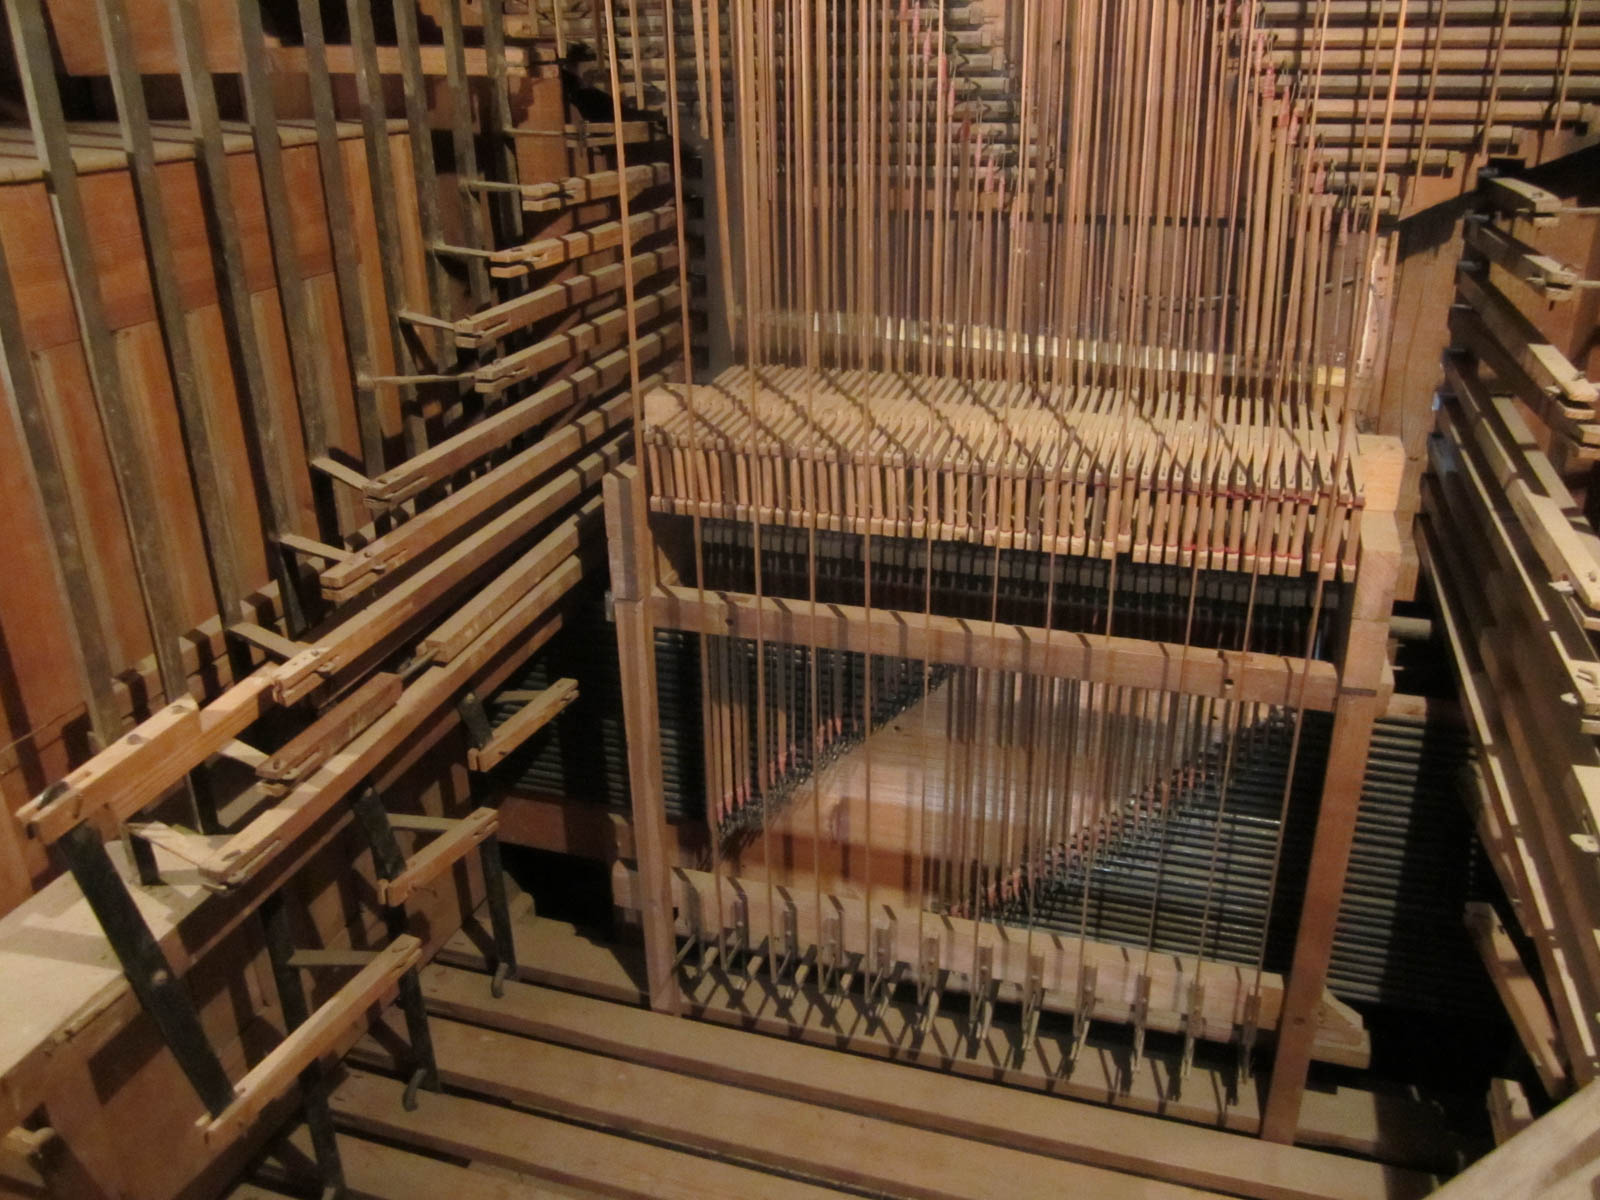
\includegraphics[width=\linewidth*3/4]{capitulo3/mecanismos}
		\par\end{centering}
	\smallskip
	\caption{\label{fig:mecanismos} Mecanismos detrás de la consola.}
\end{figure} 

\smallskip

Los entresijos del órgano barroco, el más grande, está construidos en dos plantas: en la parte más baja, a la altura de la consola, encontramos los juegos de palancas, de las cuales aquellas pertenecientes al órgano barroco suben a la planta superior. A sendos laterales encontramos el corazón del órgano romántico, más pequeño.

\smallskip

\begin{figure}[H]
	\noindent \begin{centering}
		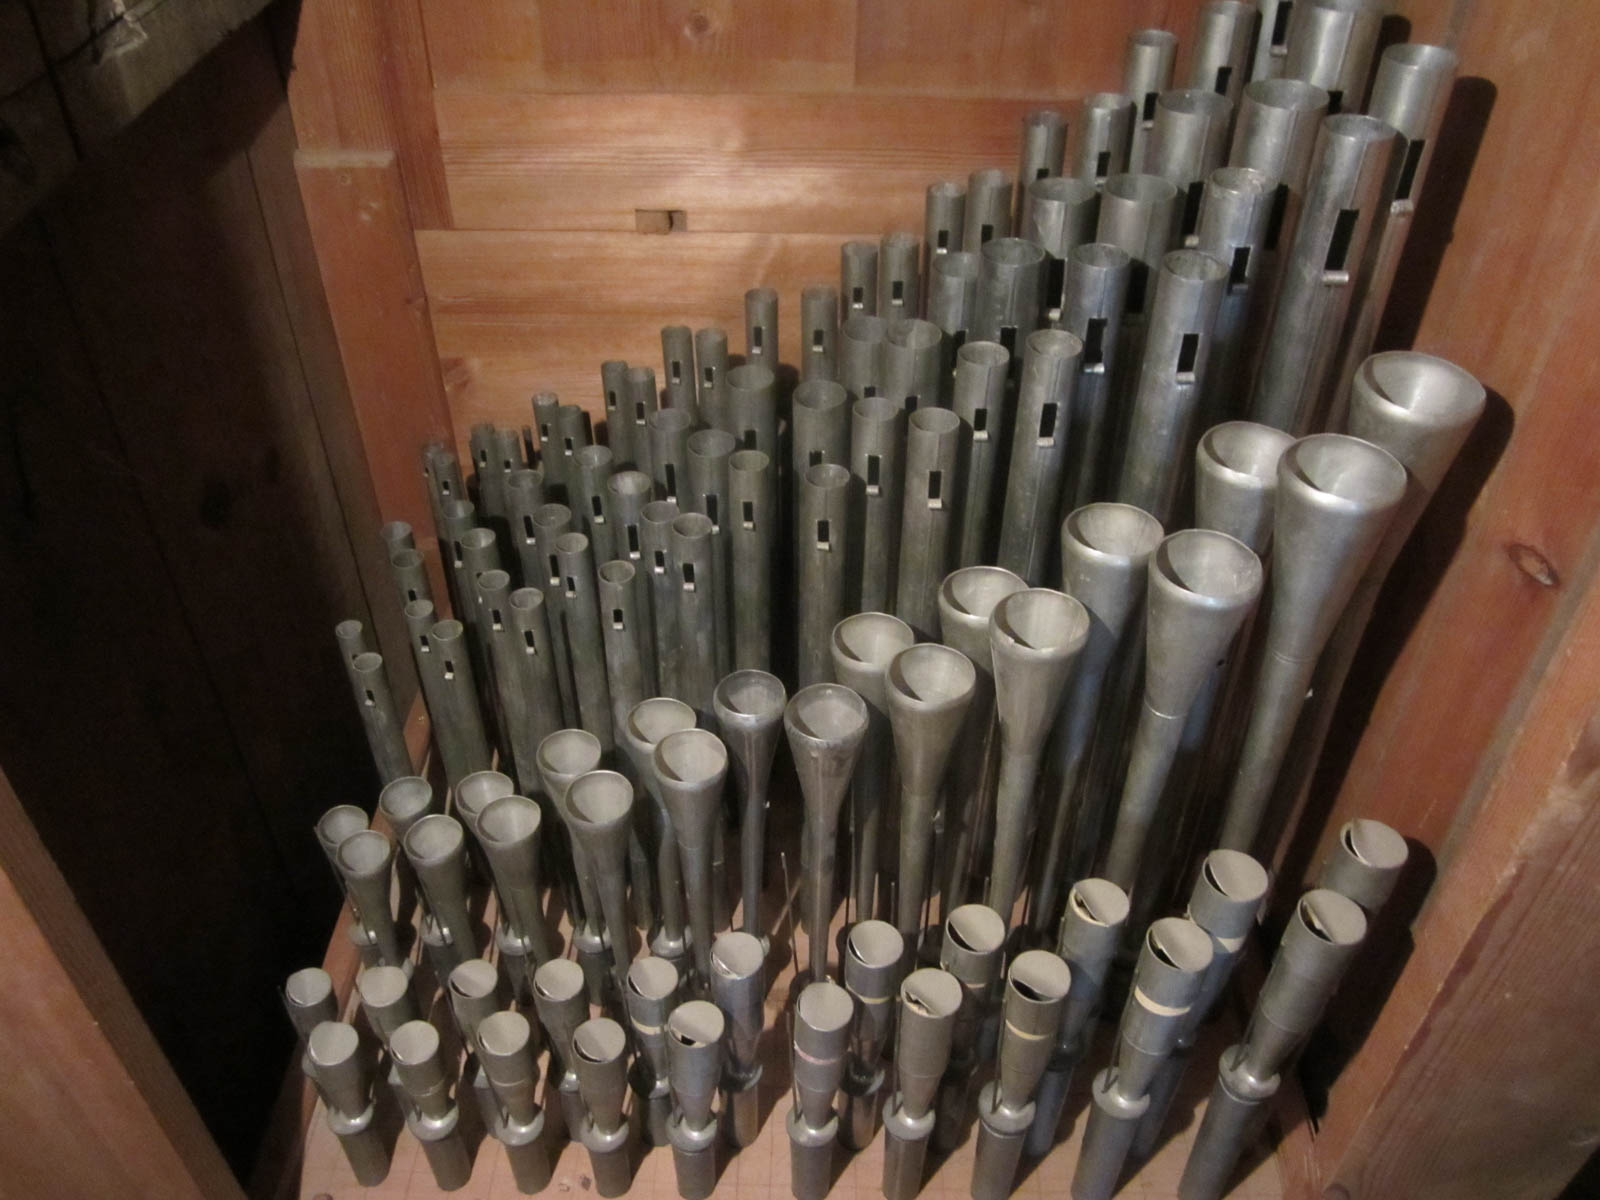
\includegraphics[width=\linewidth*2/3]{capitulo3/romantico}
		\par\end{centering}
	\smallskip
	\caption{\label{fig:romantico} Tubos del órgano romántico.}
\end{figure} 

\smallskip

En la planta de arriba se encuentra la esencia del instrumento: alrededor de 600 tubos de diferentes timbres y alturas sonoras, incluyendo el \textit{bajo de contrast}, que se hace sonar con el \textit{pedalier}. Solo los diapasones ---los flautados de 13' fundamentales y las cornetas--- son visibles desde el exterior.

\smallskip

\begin{figure}[H]
	\noindent \begin{centering}
		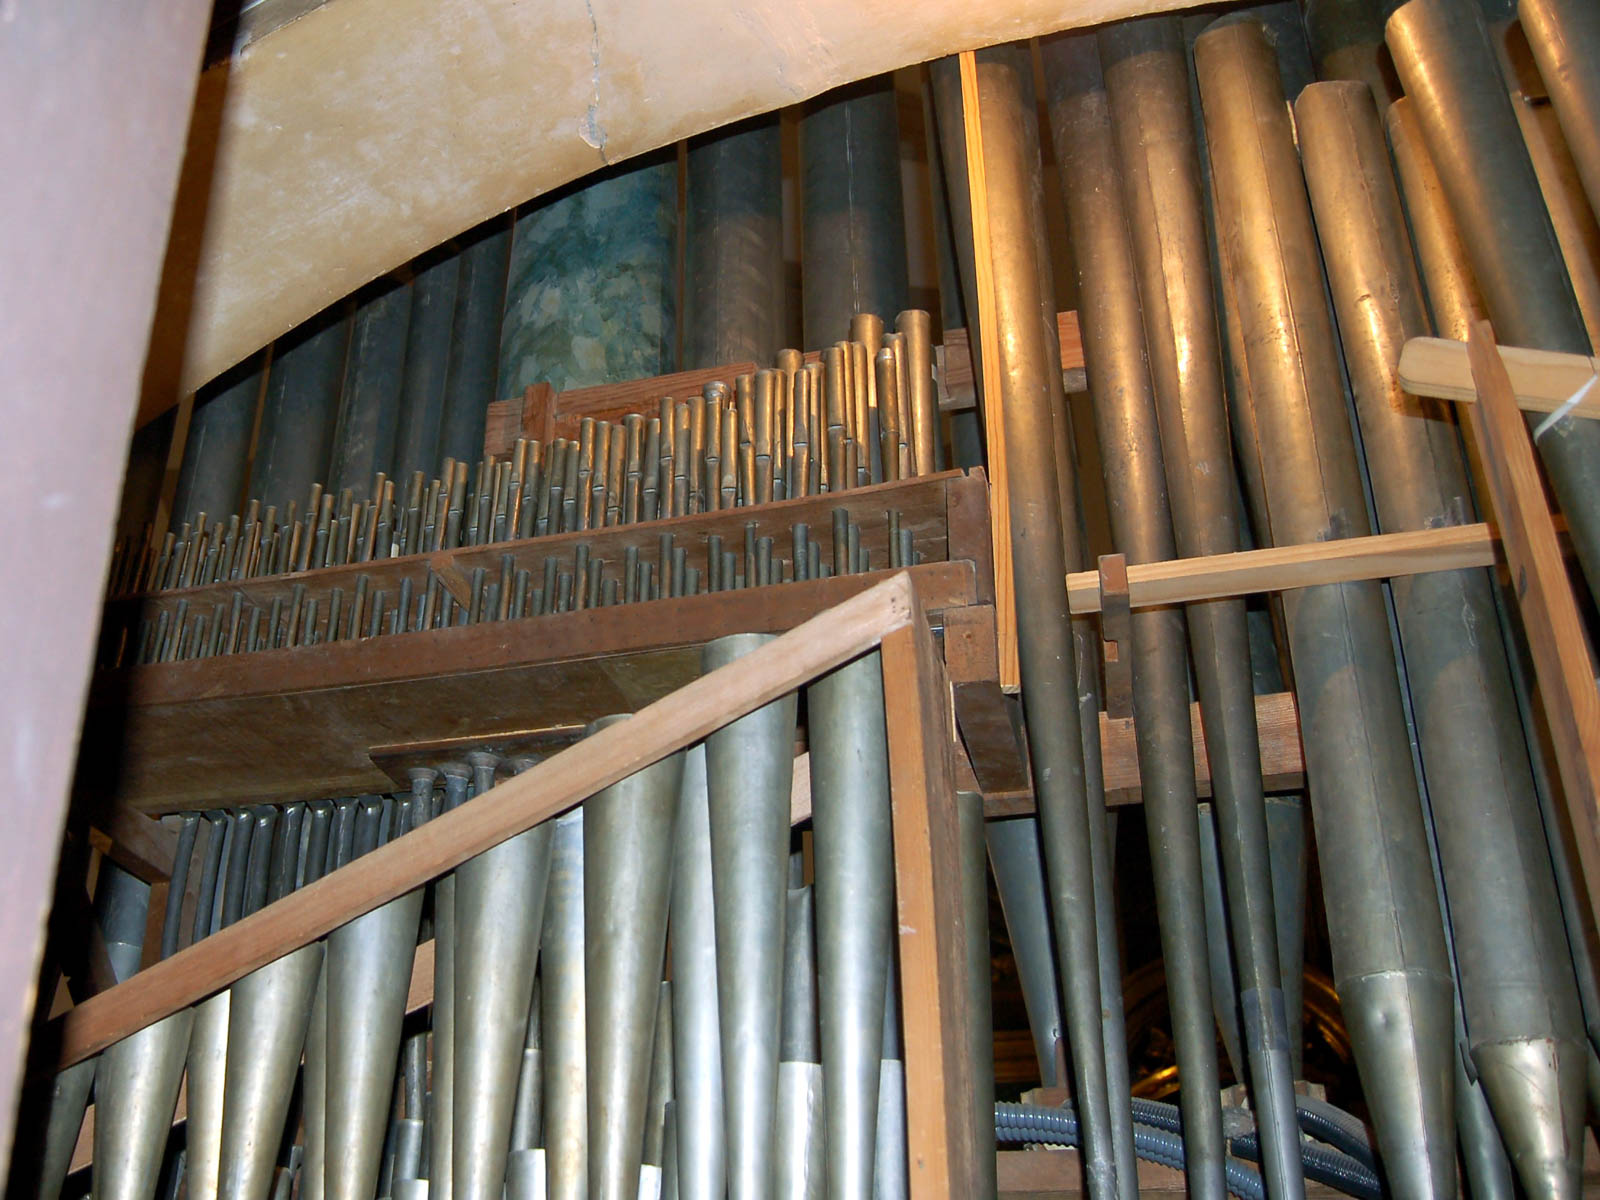
\includegraphics[width=\linewidth*2/3]{capitulo3/barroco}
		\par\end{centering}
	\smallskip
	\caption{\label{fig:barroco} Tubos del órgano barroco.}
\end{figure} 

\smallskip

La parte más importante del órgano es el llamado \textbf{secreto}, una galería a la que entra el aire procedente de la cámara de almacenamiento y se distribuye en cientos de conductos que llevan a las válvulas y los tubos. Siendo éste el corazón de la obra, dentro de él se halla una partitura firmada por el constructor del órgano. En tiempos en los que no existían los manguitos de goma, los conductos están tallados artesanalmente dentro de bloques de madera.

La primera tarea que llevamos a cabo fue conocer el órgano en profundidad, tomar algunas medidas y diseñar el modelo en 3D con el \textit{software} \textit{SolidWorks}.

\subsection{Teclados}

Tenemos dos teclados de cuatro octavas notas cada uno, el de arriba, correspondiente al órgano barroco, y otro más abajo, que sobresale del primero, para el órgano romántico, de la misma extensión.

\smallskip

\begin{figure}[H]
	\noindent \begin{centering}
		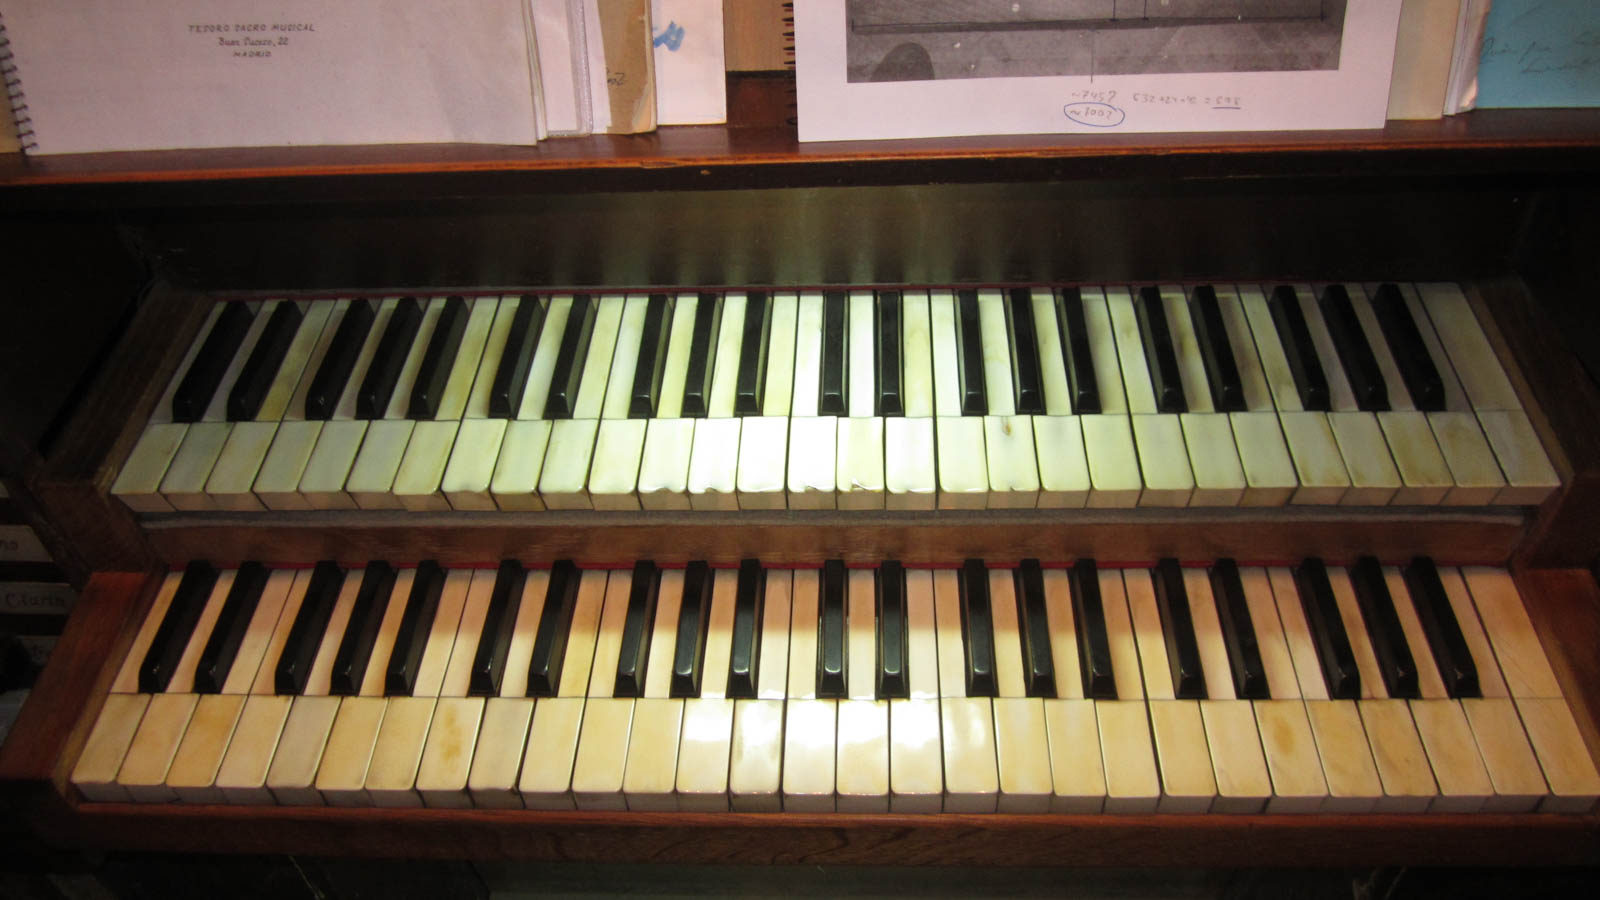
\includegraphics[width=\linewidth*3/4]{capitulo3/teclados}
		\par\end{centering}
	\smallskip
	\caption{\label{fig:teclados} Teclados del órgano.}
\end{figure} 

\smallskip

Tanto las medidas de cada tecla como su calado (diferencia entre la posición del borde de una tecla pulsada y sin pulsar) son estándar y coincidentes con las del piano. De la misma forma, la tecla \textit{Do} del centro hace sonar la nota \textit{Do 4} \footnotemark.

\footnotetext{En España se utilizan dos índices de notación musical: el franco-belga, que asigna el nombre \textit{La 3} a la nota cuya frecuencia fundamental vibra a 440 \textit{Hz}, y el índice científico, que asigna \textit{La 4} a la misma nota. En este proyecto utilizaremos el índice científico, ya que es el utilizado para el sistema \acrshort{MIDI}.}

Los datos más relevantes son los siguientes:

\smallskip

\begin{center}
	\begin{tabular}{|l|l|}
		\hline Número de teclas & 49 / teclado \\
		\hline Extensión & \textit{Do 2} -- \textit{Do 6} \\
		\hline Profundidad de calado (blancas) & 10 \textit{mm} \\
		\hline Profundidad de calado (negras) & 8 \textit{mm} \\
		\hline Presión máxima & 2,70 \textit{N} \\
		\hline
	\end{tabular}
	\smallskip
	\captionof{table}{\label{tab:teclados} Medidas de los teclados.}
\end{center}

\smallskip

Cada tecla blanca del mismo nombre tiene unas medidas ligeramente diferentes en su parte interna, para permitir que las negras encajen perfectamente. Las medidas de una tecla blanca son las siguientes:

\smallskip

\begin{figure}[H]
	\noindent \begin{centering}
		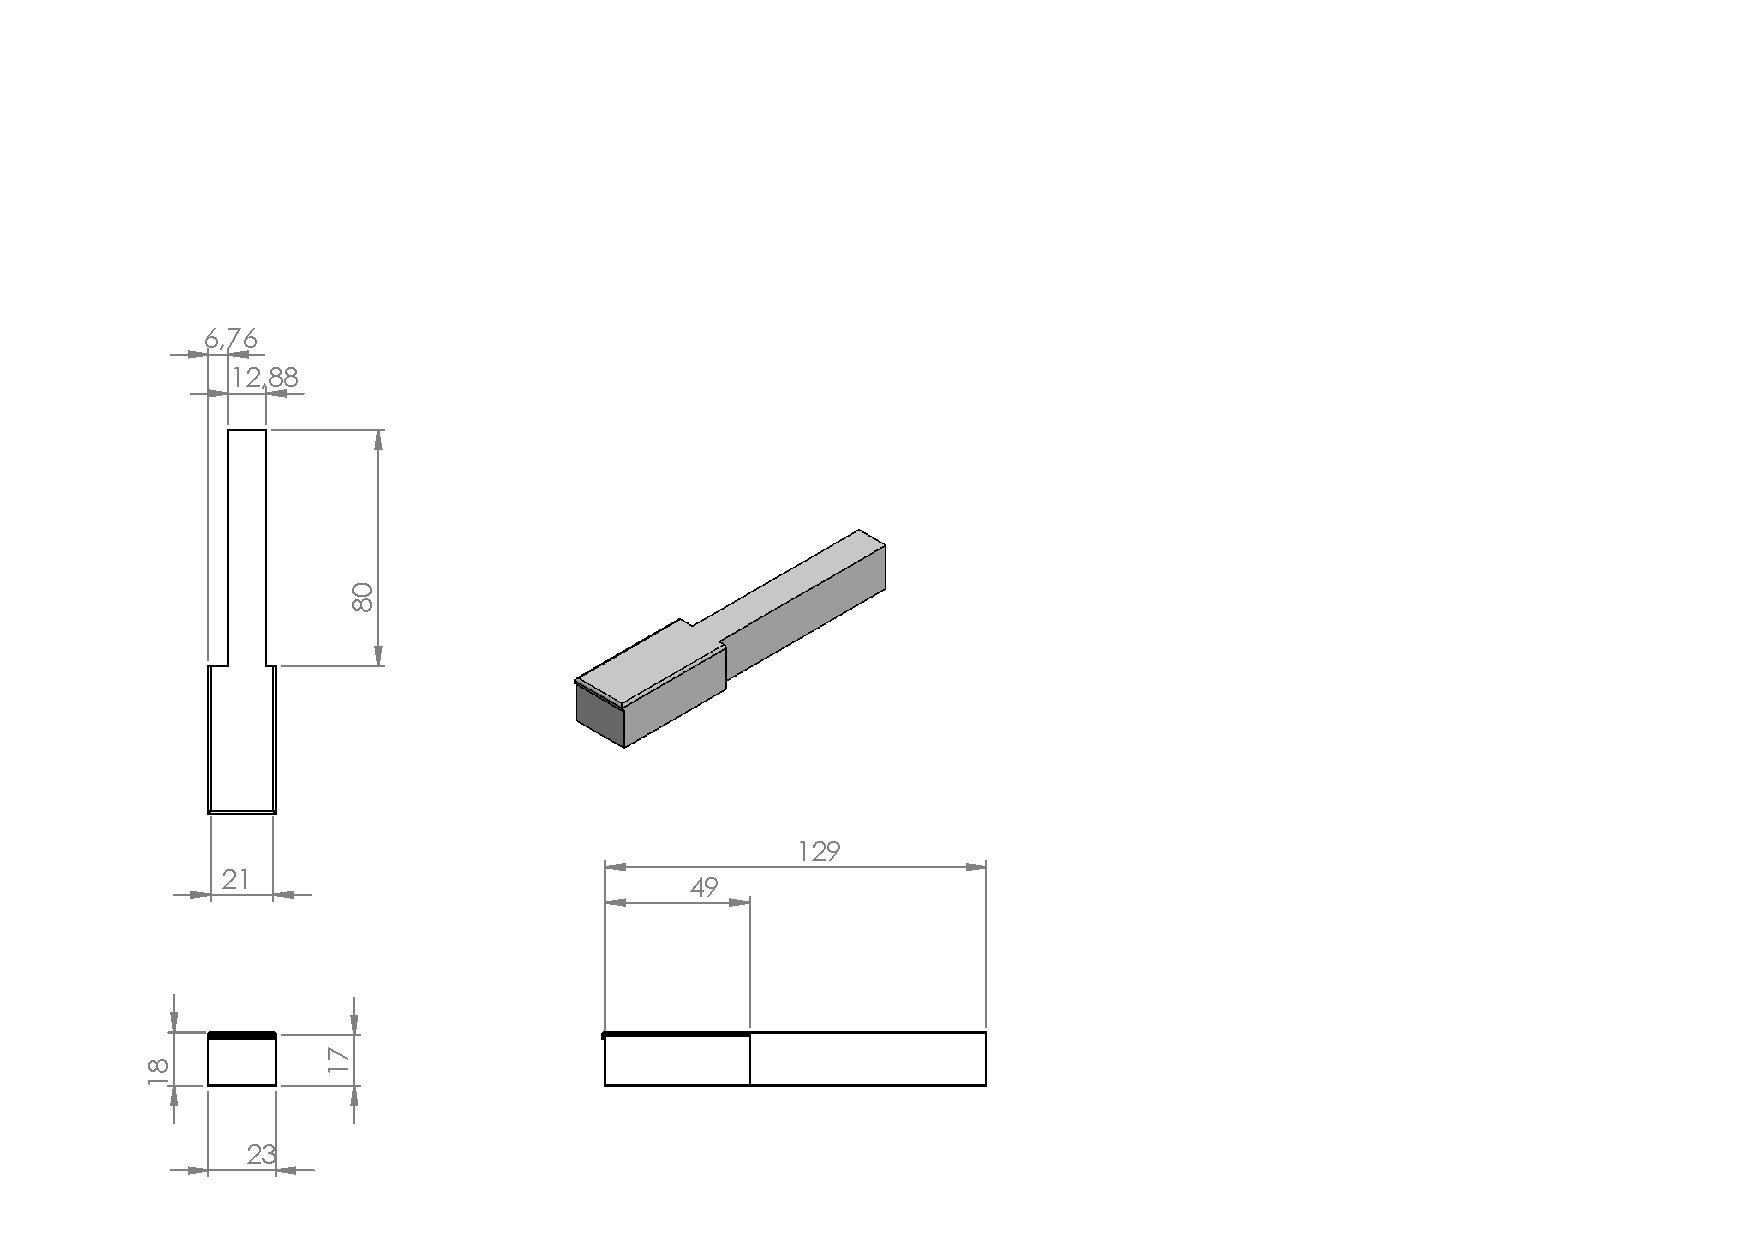
\includegraphics[clip=true,trim=0 0 360 150, width=\linewidth/2]{capitulo3/blanca_modelo}
		\par\end{centering}
	\smallskip
	\caption{\label{fig:blanca_modelo} Medidas de una tecla blanca.}
\end{figure} 

\smallskip

Las teclas negras, en cambio, son más cortas y más delgadas, sobresaliendo del teclado entre las blancas. Producen las notas cromáticas.

\smallskip

\begin{figure}[H]
	\noindent \begin{centering}
		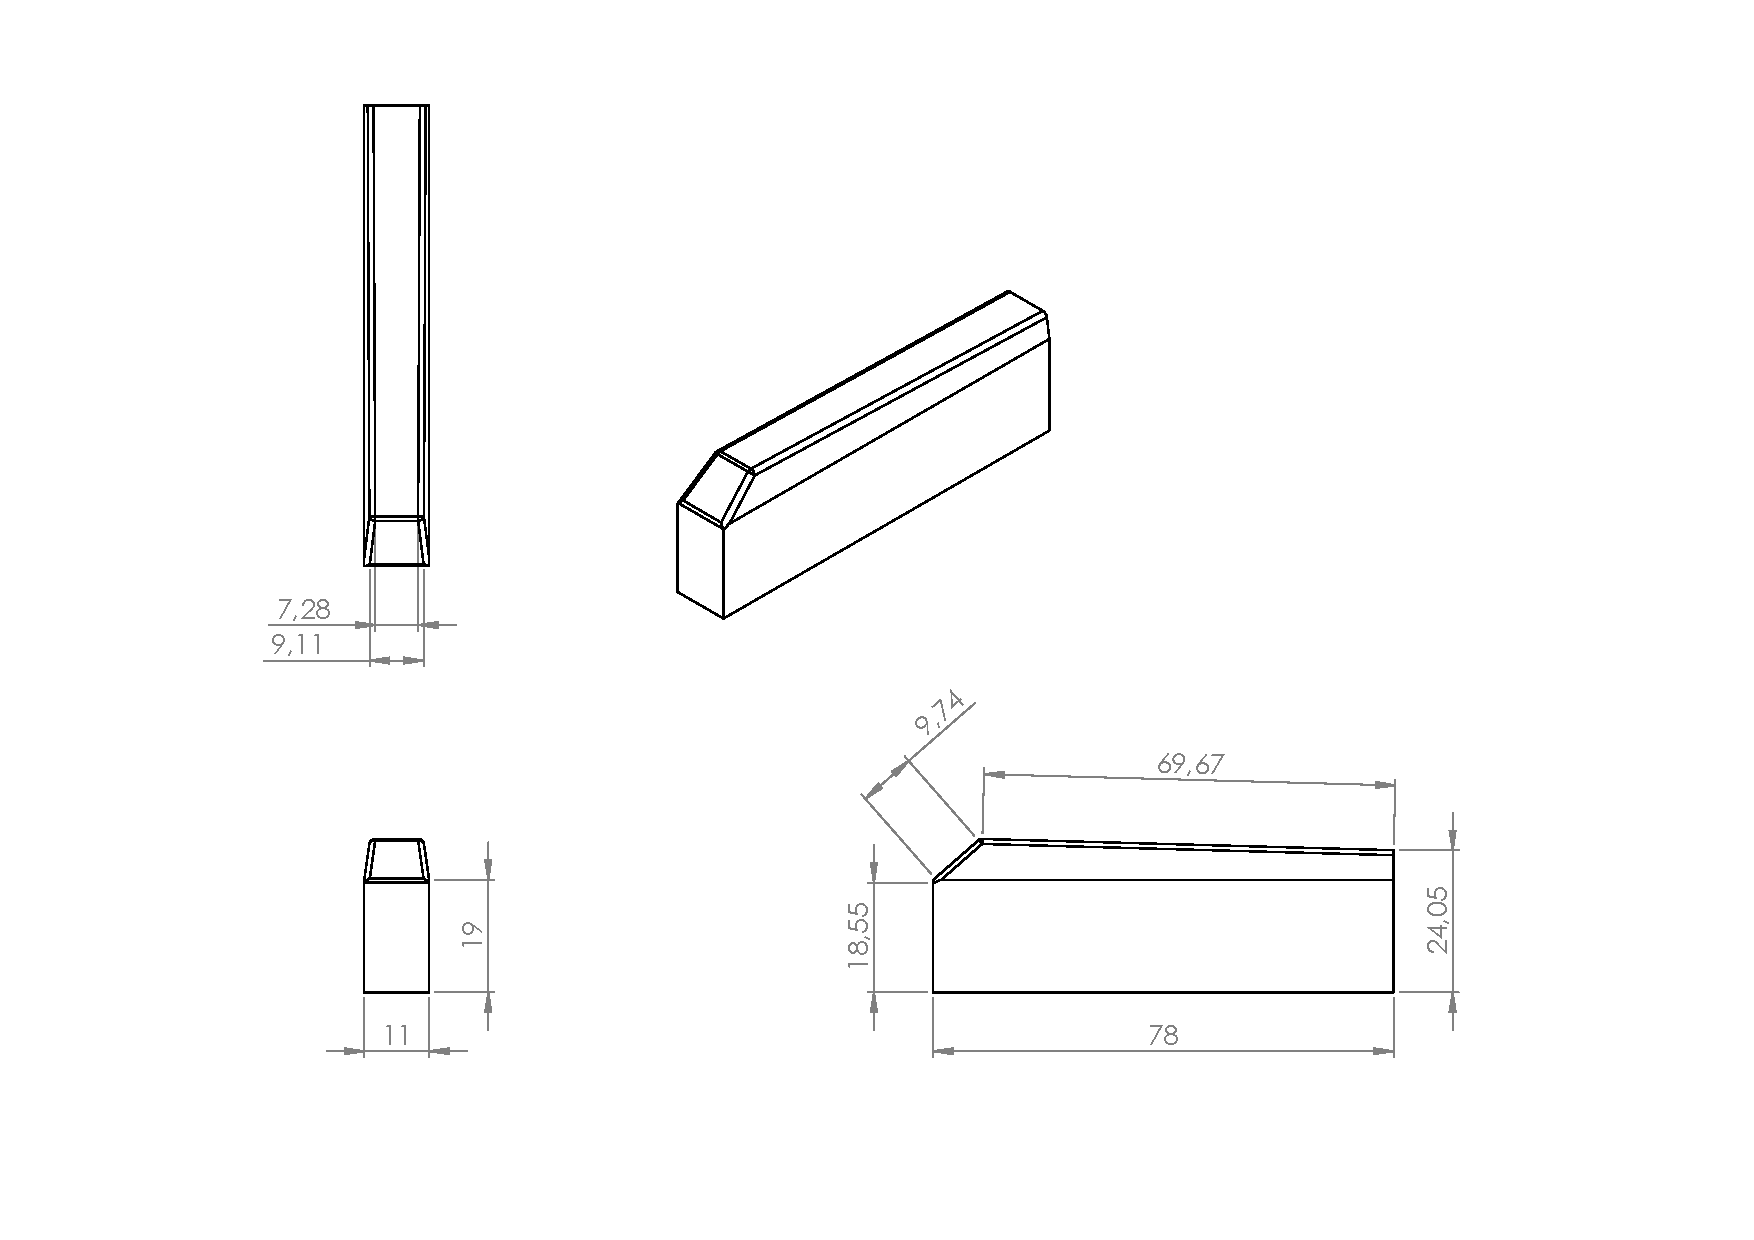
\includegraphics[clip=true,trim=50 50 50 50, width=\linewidth/2]{capitulo3/negra_modelo}
		\par\end{centering}
	\smallskip
	\caption{\label{fig:negra_modelo} Medidas de una tecla negra.}
\end{figure} 

\smallskip

A continuación presentamos las medidas tomadas sobre el teclado en conjunto:

\smallskip

\begin{figure}[H]
	\noindent \begin{centering}
		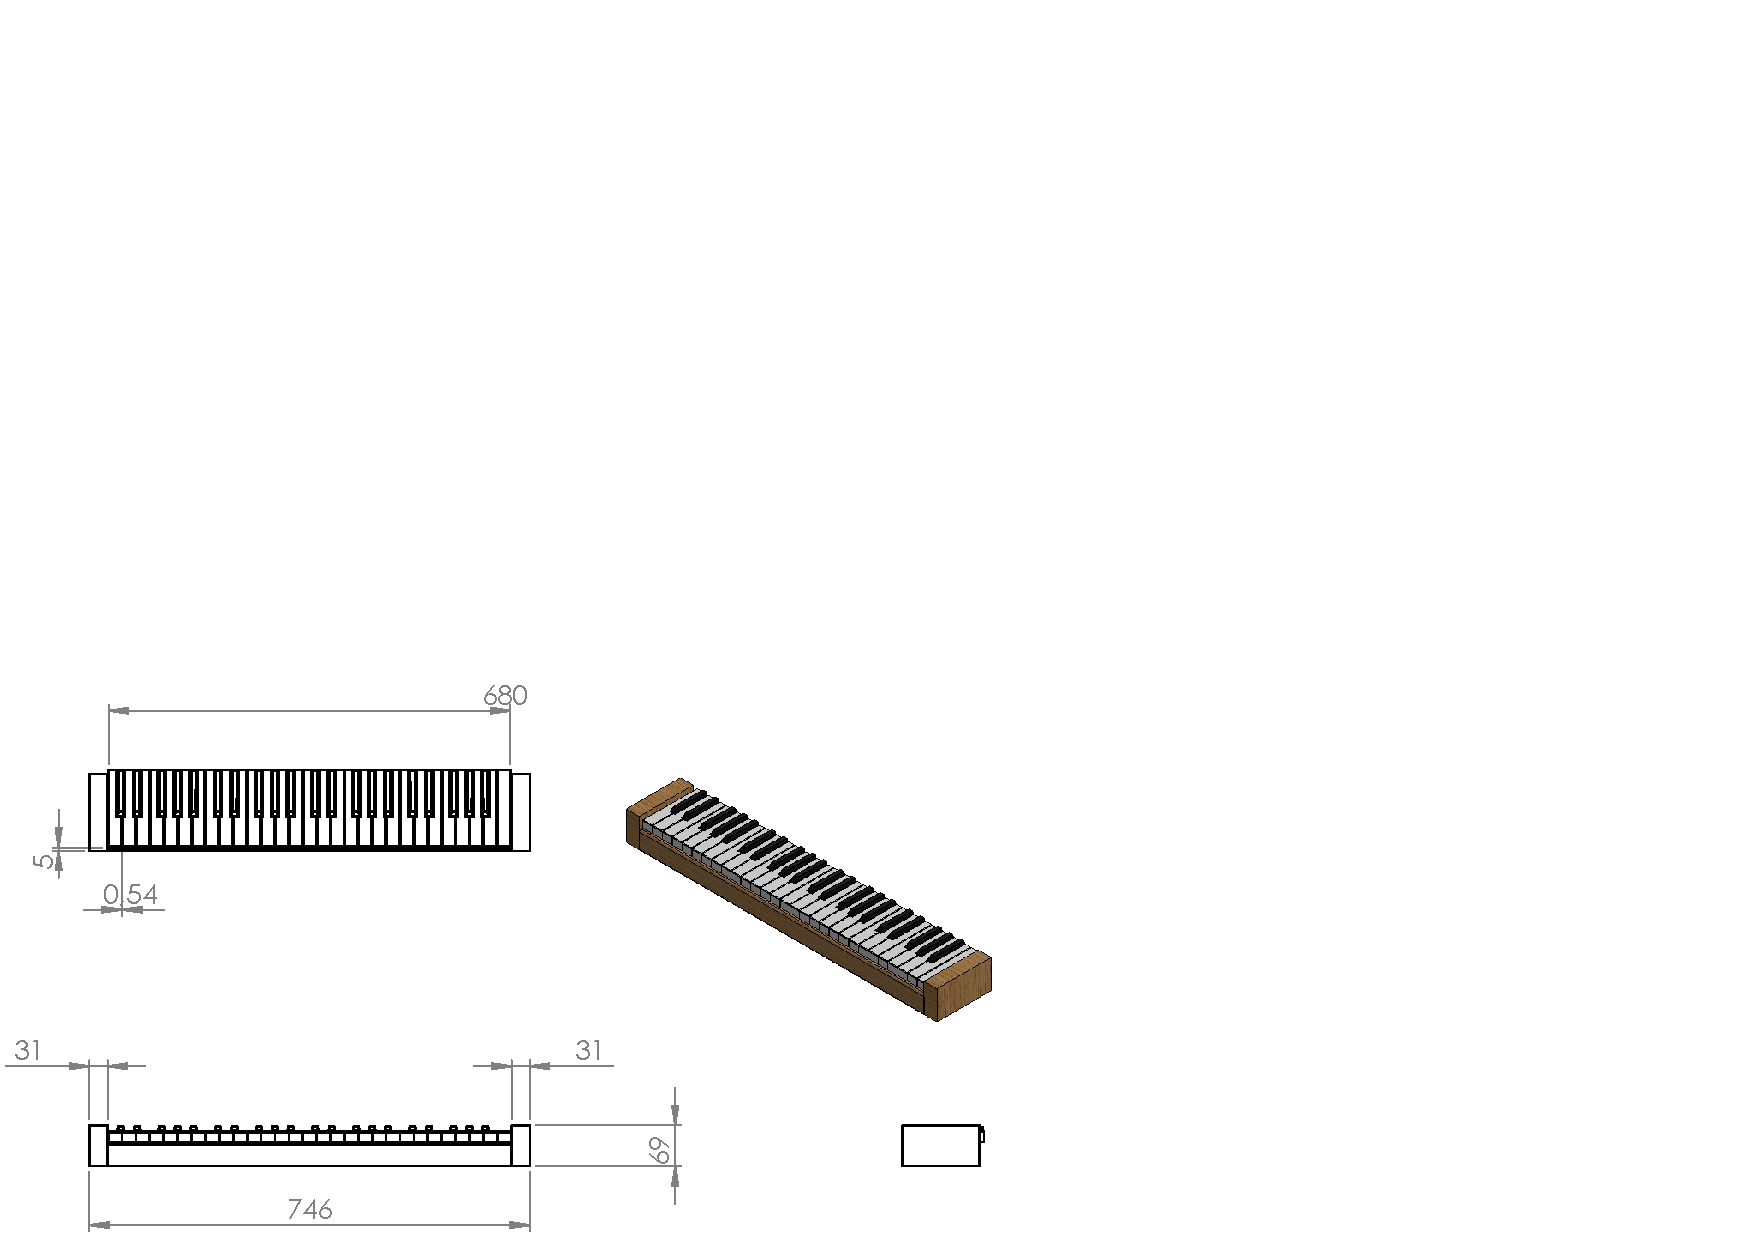
\includegraphics[clip=true,trim=0 0 360 320, width=\linewidth*3/4]{capitulo3/teclado_modelo}
		\par\end{centering}
	\smallskip
	\caption{\label{fig:teclado_modelo} Medidas del teclado.}
\end{figure} 

\smallskip

Cabe destacar que, a diferencia del piano, la intensidad del sonido no viene dada por la fuerza con la que se pulse una tecla, y no es necesario pulsarla hasta el tope de calado para que suene, basta con hacerla bajar tan solo unos milímetros, lo necesario para vencer la válvula.

\subsection{Pedales}

Este órgano cuenta con un \textit{pedalier} con un registro fijo: el \textit{bajo de contrast}. Los pedales están dispuestos en forma de escala diatónica, igual que las teclas. Cada pedal tiene aproximadamente la misma anchura que una tecla aunque, obviamente, están más separados unos de otros.

\smallskip

\begin{figure}[H]
	\noindent \begin{centering}
		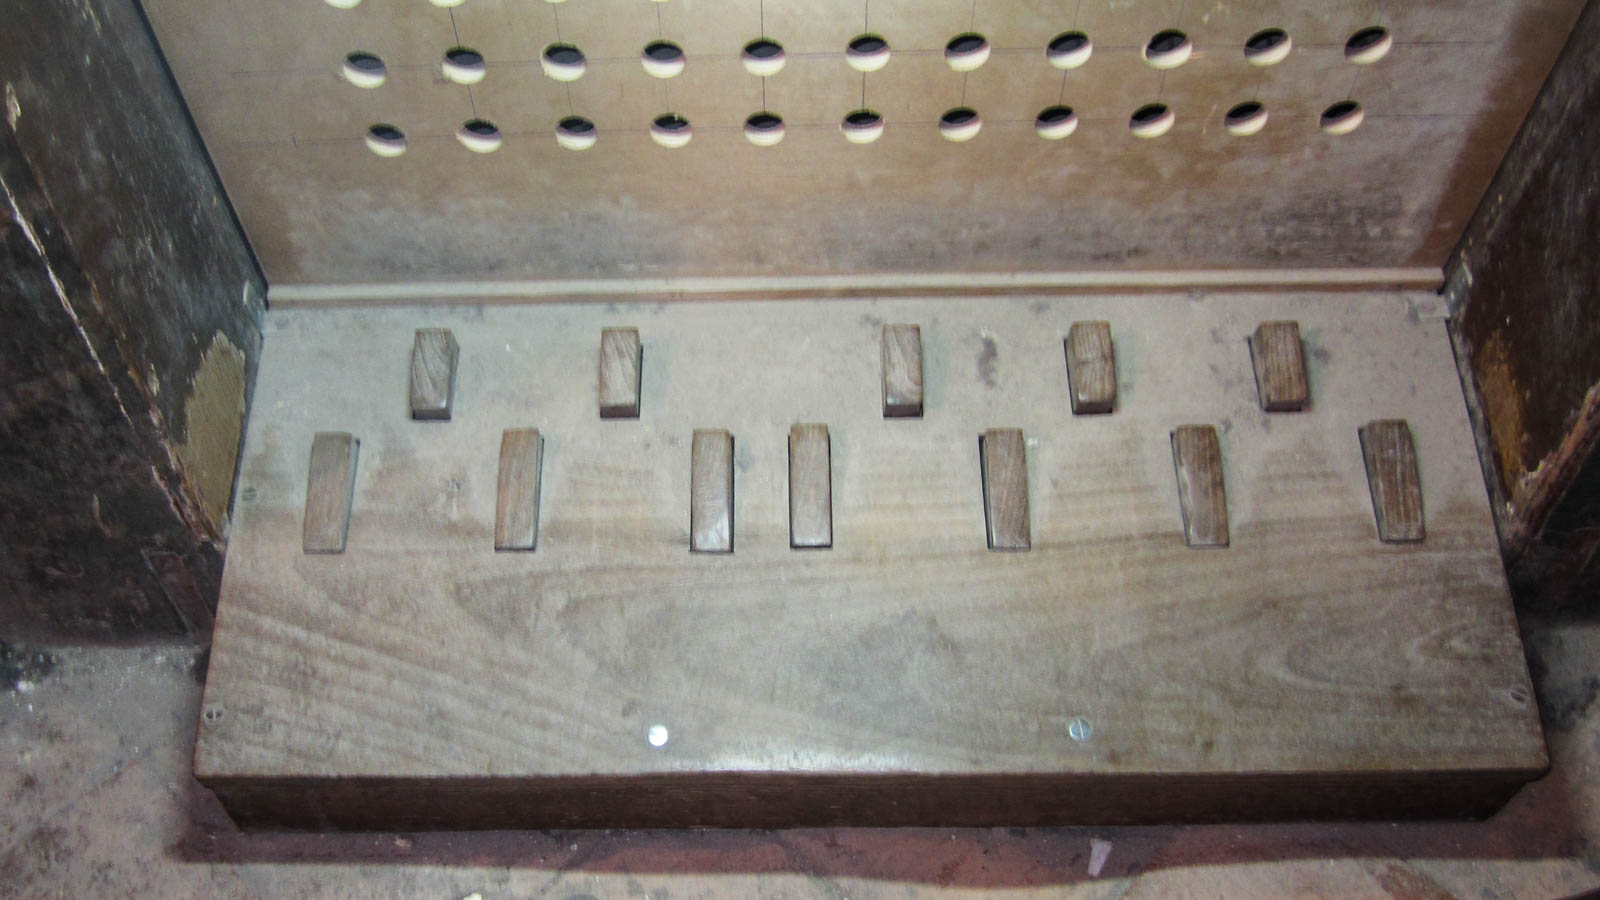
\includegraphics[width=\linewidth*3/4]{capitulo3/pedalier}
		\par\end{centering}
	\smallskip
	\caption{\label{fig:pedalier} \textit{Pedalier} del órgano.}
\end{figure} 

\smallskip

Es importante saber que el peso necesario para mover un pedal es mucho mayor que para una tecla, asimismo, tanto la naturaleza artesanal como el deterioro crean mucha disparidad entre el tacto de cada pedal.

\smallskip

\begin{center}
	\begin{tabular}{|l|l|}
		\hline Número de pedales & 12 \\ 
		\hline Extensión & \textit{Do 1} -- \textit{Si 1} \\ 
		\hline Profundidad de calado (diatónicas) & 14,5 \textit{mm} \\ 
		\hline Profundidad de calado (cromáticas) & 19,8 \textit{mm} \\
		\hline Presión máxima & 30,54 \textit{N} \\
		\hline 
	\end{tabular}
	\smallskip
	\captionof{table}{\label{tab:pedalier} Medidas del \textit{pedalier}.}
\end{center}

\smallskip

Por su parte, las cotas que definen el \textit{pedalier} son las siguientes:

\smallskip

\begin{figure}[H]
	\noindent \begin{centering}
		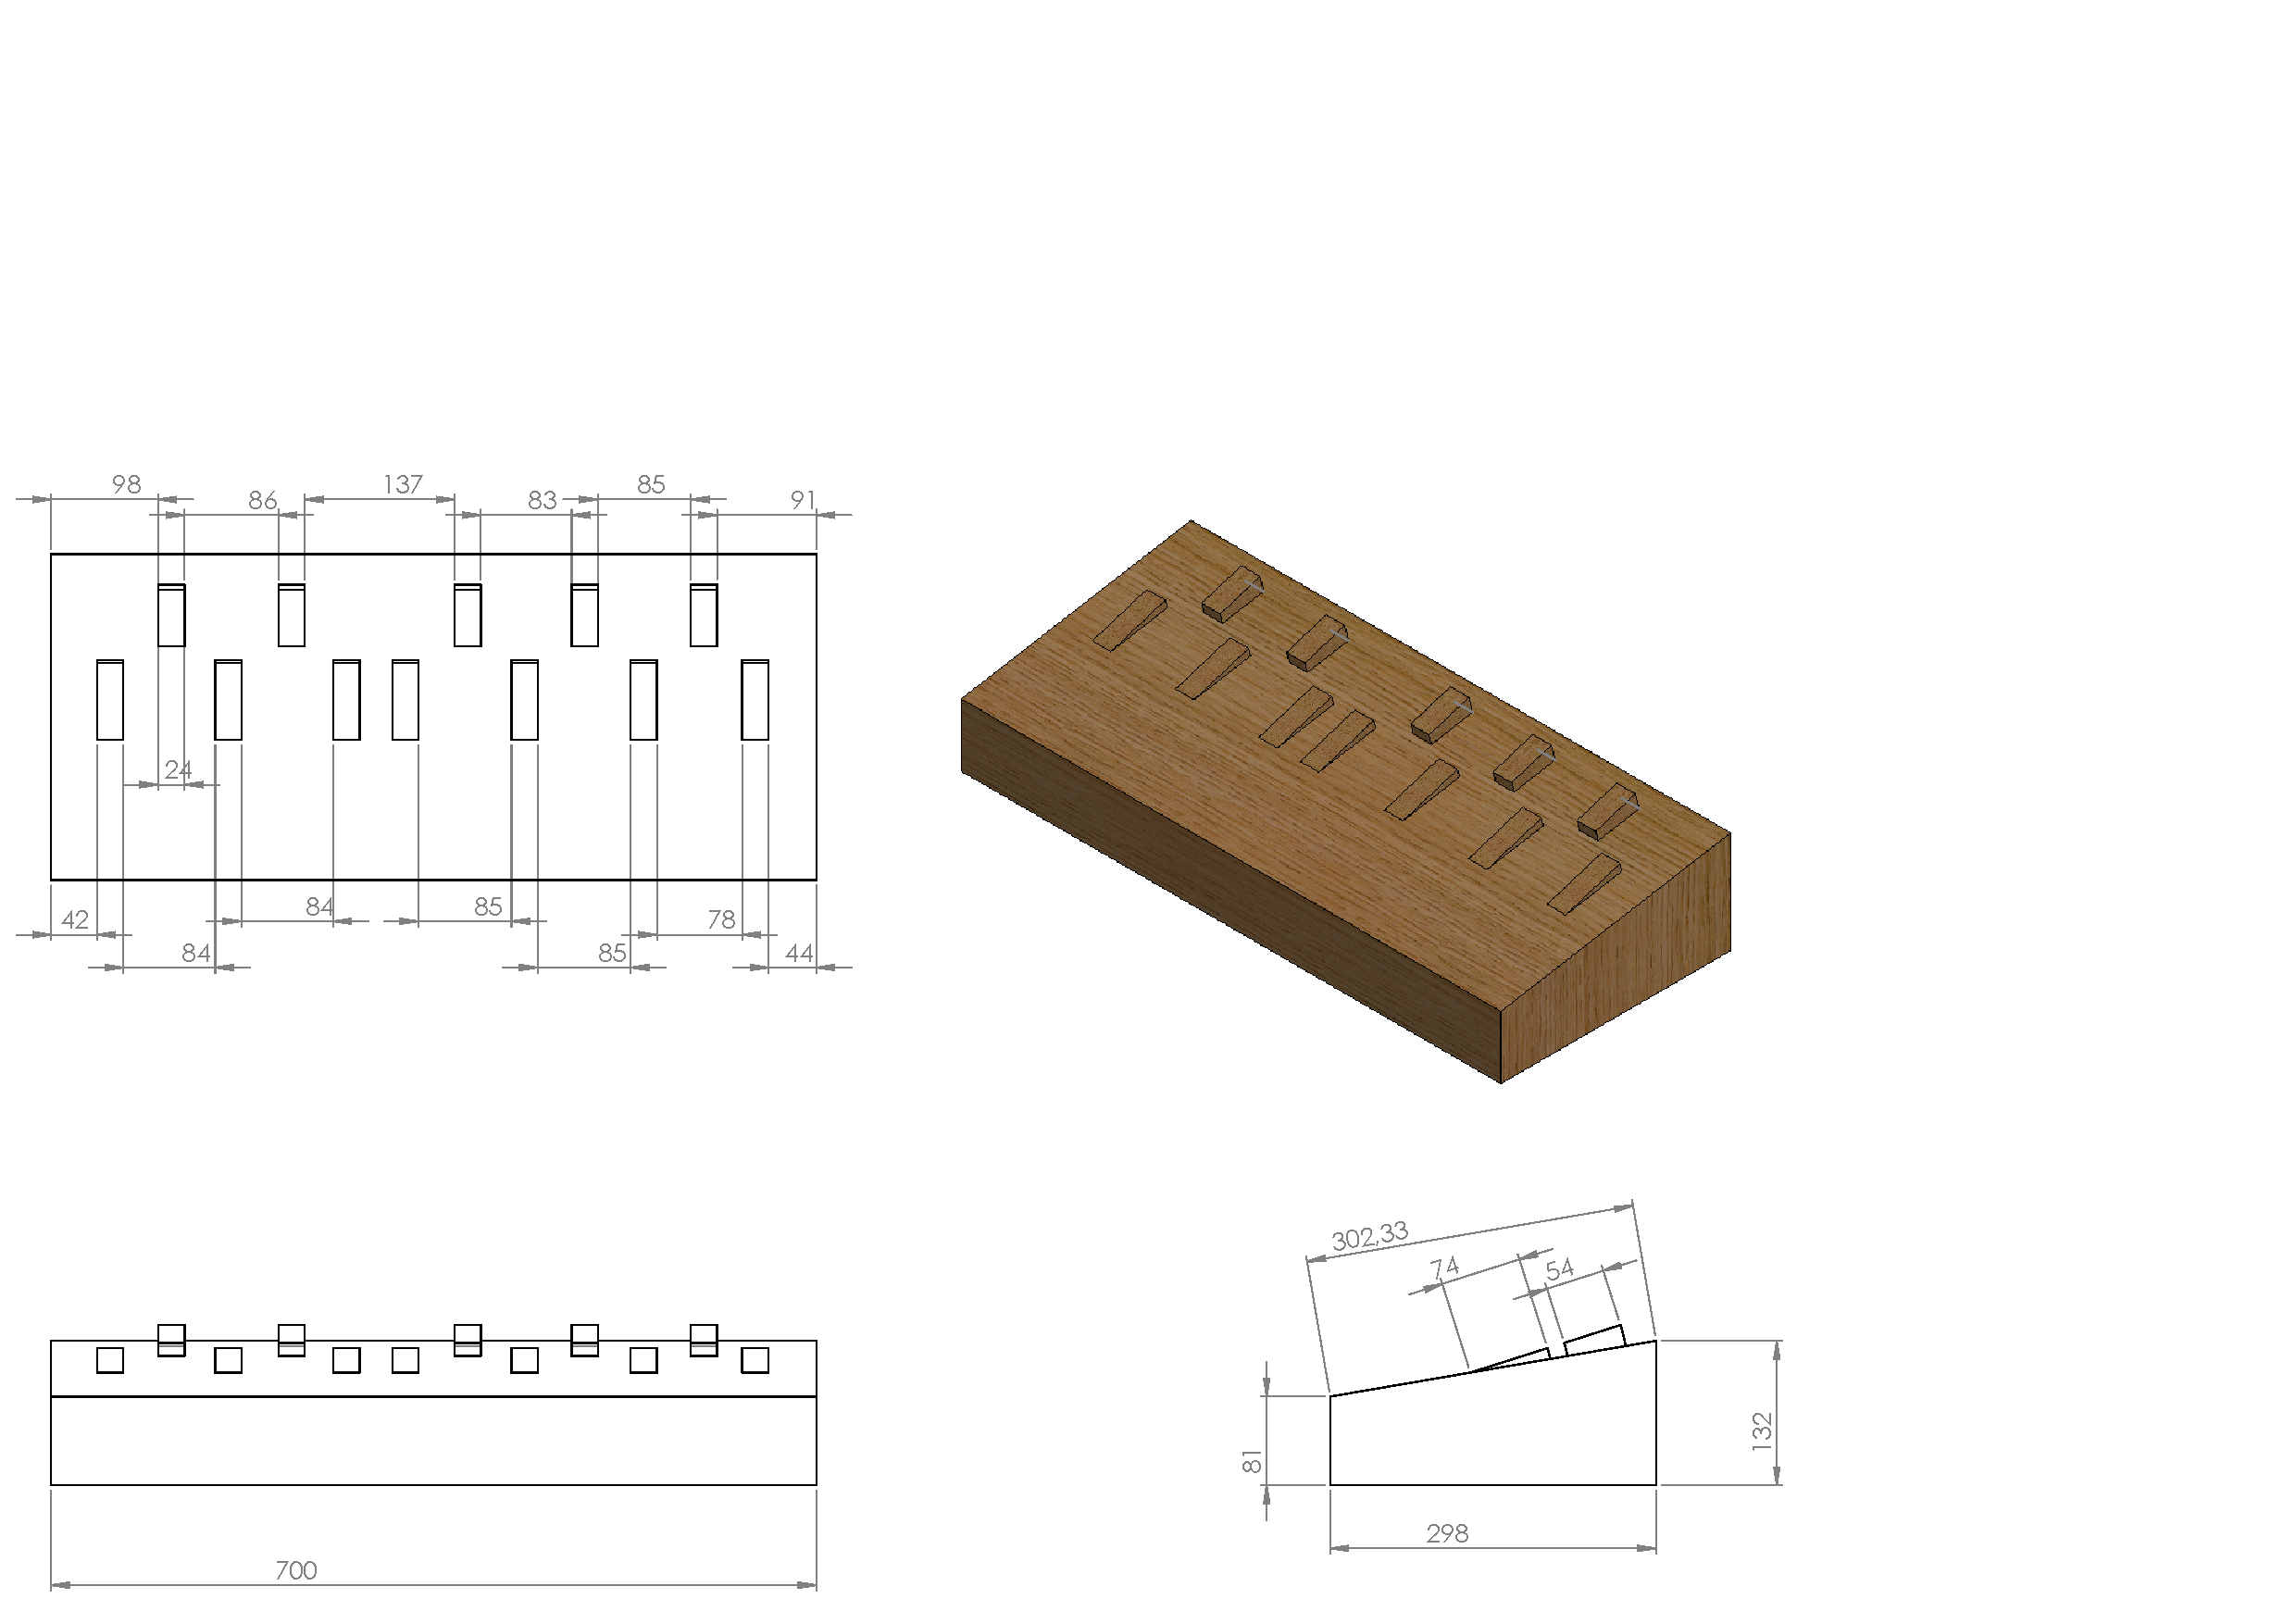
\includegraphics[clip=true,trim=0 0 260 250, width=\linewidth*3/4]{capitulo3/pedalier_modelo}
		\par\end{centering}
	\smallskip
	\caption{\label{fig:pedalier_modelo} Medidas de los pedales.}
\end{figure} 

\smallskip

\subsection{Registros}

Los registros son las diferentes familias de tubos con el mismo timbre y la misma tesitura. Se pueden abrir o cerrar desde la consola a través de una serie de palancas, de las que se tira para hacer sonar el registro o se empuja para silenciarlo.

\smallskip

\begin{figure}[H]
	\noindent \begin{centering}
		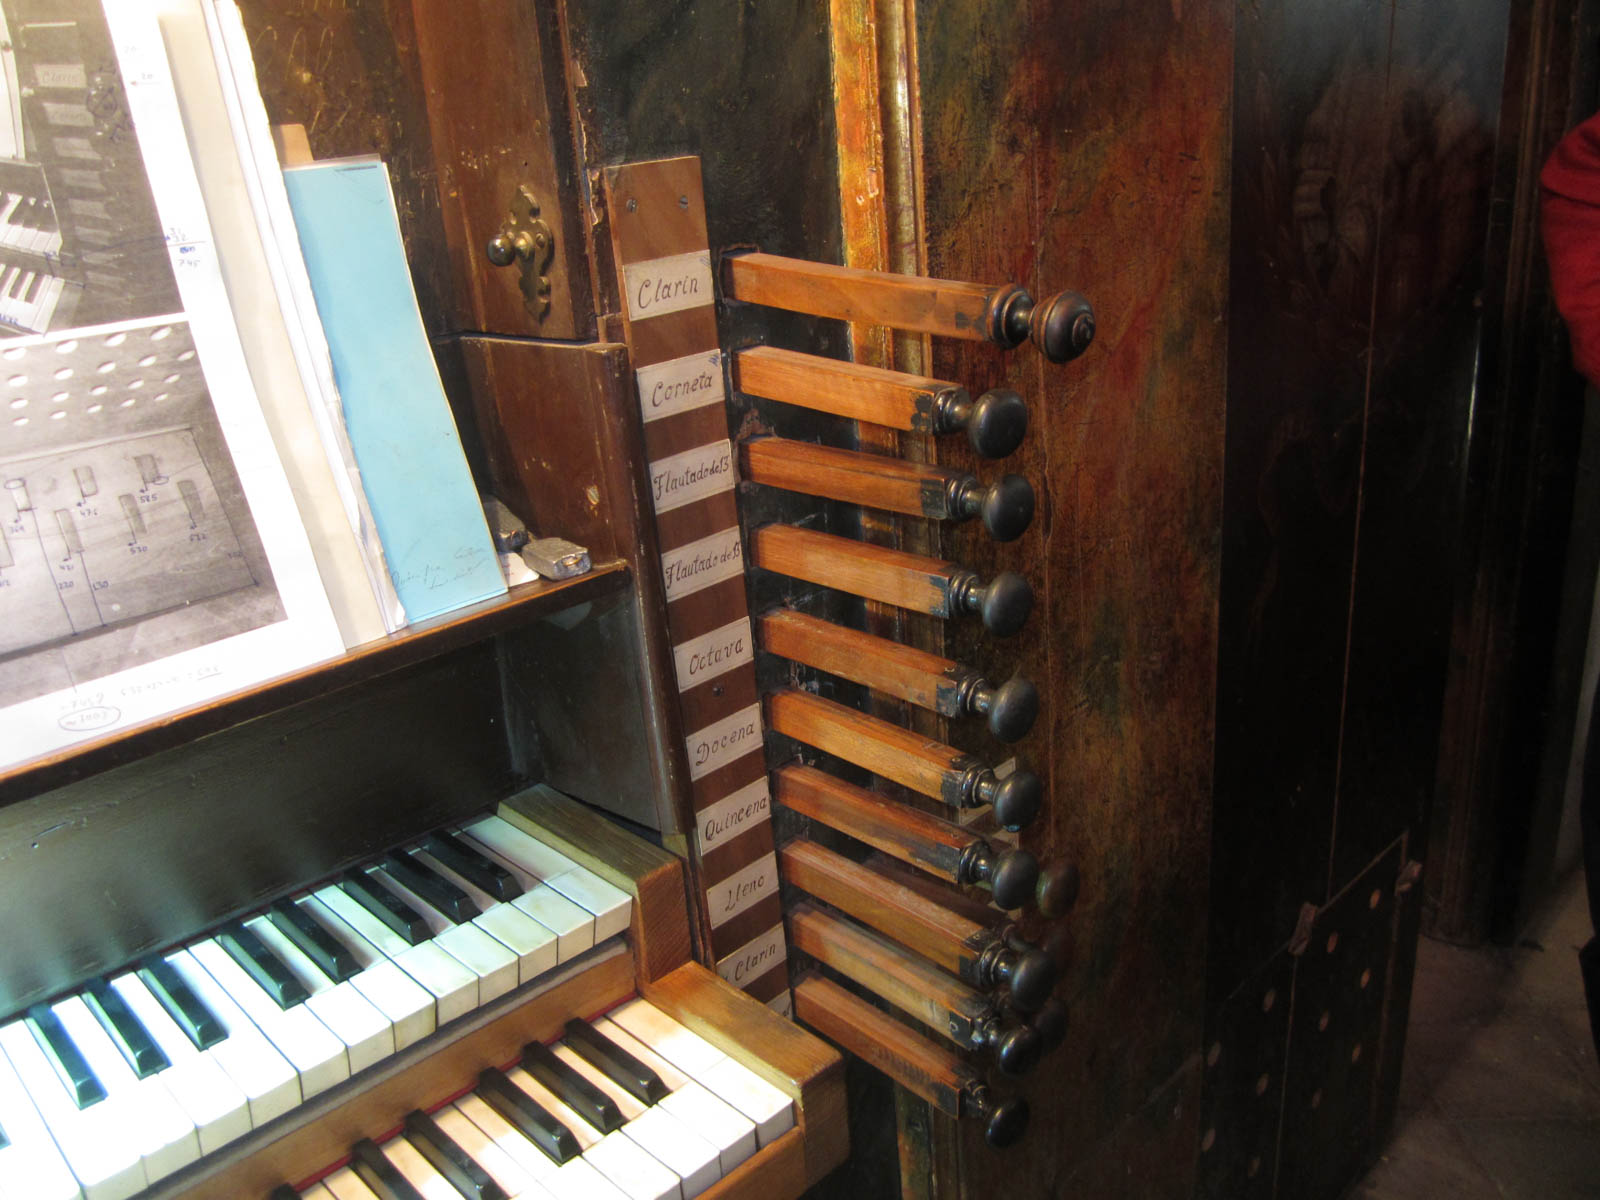
\includegraphics[width=\linewidth*2/3]{capitulo3/registros}
		\par\end{centering}
	\smallskip
	\caption{\label{fig:registros} Registros a la derecha del teclado.}
\end{figure} 

\smallskip

Estos controles están dispuestos a ambos lados de los teclados y son exclusivos para un teclado u otro. En este órgano existen registros parciales, esto es, se aplican solo a una mitad del teclado, bien de \textit{Do 2} a \textit{Si 3}, o bien de \textit{Do 4} a \textit{Do 6}.

Dado que el punto interno de equilibro de cada palanca está en lugares diferentes, existe una notable disparidad en la medida en que sobresalen cuando se abren. Además, tenemos una palanca especial, el \textit{tremolo}, que sirve para activar un mecanismo que produce un efecto de fluctuación en el sonido.

A continuación mostramos las medidas de longitud tomadas durante el análisis.

\smallskip

\begin{center}
	\begin{tabular}{|l|l|}
		\hline \multicolumn{2}{|c|}{\textbf{A la izquierda}} \\	
		\hline & Bajoncillo (142 \textit{mm}) \\ 
		\hline & Flautado de 13' sordina (160 \textit{mm}) \\ 
		\hline & Flautado de 13' (175 \textit{mm})\\ 
		\hline & Octava (161 \textit{mm}) \\ 
		\hline & Quincena (161 \textit{mm}) \\ 
		\hline Trémolo (67 \textit{mm}) & Decimonovena (165 \textit{mm}) \\ 
		\hline Bajón-oboe (103 \textit{mm}) & Lleno (140 \textit{mm})  \\ 
		\hline Flauta armenia (1106 \textit{mm}) & Clarín (160 \textit{mm}) \\ 
		\hline  Violón (100 \textit{mm}) & Trompeta real (144 \textit{mm})  \\ 
		\hline
	\end{tabular}
	\smallskip
	\captionof{table}{\label{tab:registros_izquierda} Medidas de los registros (izquierda).}
\end{center}

\smallskip
	
\begin{center}
	\begin{tabular}{|l|l|}
		\hline \multicolumn{2}{|c|}{\textbf{A la derecha}} \\
		\hline Clarín (170 \textit{mm}) &  \\ 
		\hline Corneta (141 \textit{mm}) &  \\ 
		\hline Flautado de 13' sordina (137 \textit{mm}) &  \\ 
		\hline Flautado de 13' (134 \textit{mm}) &  \\ 
		\hline Octava & (142 \textit{mm}) \\ 
		\hline Docena & (142 \textit{mm}) \\ 
		\hline Quincena & (168 \textit{mm}) \\ 
		\hline Lleno (156 \textit{mm}) & Voz humana (110 \textit{mm}) \\ 
		\hline Clarín (142 \textit{mm}) & Voz celeste (116 \textit{mm}) \\ 
		\hline Trompeta real (135 \textit{mm}) & Gamba (102 \textit{mm}) \\ 
		\hline 
	\end{tabular}
	\smallskip
	\captionof{table}{\label{tab:registros_derecha} Medidas de los registros (derecha).}
\end{center}

\smallskip

\section{PCB de control}

La placa de circuito impreso es la solución a los requisitos \textit{hardware} aportada por el proyecto de D. Mikel Aguayo Fernández \cite{mikel}. Incluye una serie de registros de desplazamiento para almacenar el estado del órgano, una interfaz de control local reducido y un medio de control remoto. También alimentará al computador que vamos a utilizar. Actualmente disponemos de un prototipo de la placa con un número limitado de salidas.

Una de las partes más importantes de este proyecto será desarrollar el \textit{software} controlador para esta \acrshort{PCB}. A continuación detallamos aquellos componentes con los que tendremos que interactuar.

\subsection{Registros de desplazamiento SN74HC595}

Los registros de desplazamiento son circuitos lógicos que almacenan una serie de bits y permiten desplazarlos de una celda a otra. Este modelo tiene una capacidad de 8 bits, soporta entrada en serie y salida en paralelo con registro de almacenamiento \cite{shiftreg}. 

Así, solo necesitamos un pin para enviar toda la información, y la salida no se ve alterada durante el desplazamiento, sino que damos un pulso de reloj para indicar que hemos terminado de enviar los datos.

\smallskip

\begin{figure}[H]
	\noindent \begin{centering}
		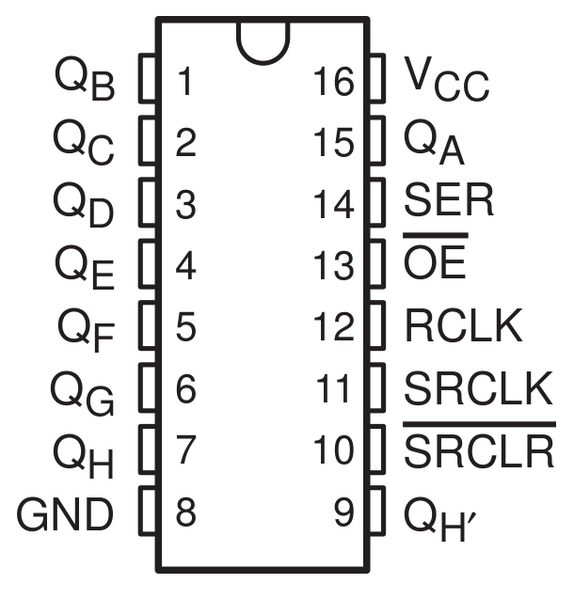
\includegraphics[width=\linewidth/4]{capitulo3/SN74HC595}
		\par\end{centering}
	\smallskip
	\caption{\label{fig:SN74HC595} Pines del SN74HC595. }
\end{figure} 

\smallskip

La información más relevante es la siguiente:

\smallskip

\begin{center}
		\begin{tabular}{|l|l|}
		\hline Capacidad & 8 \textit{bits} / canal \\ 
		\hline Canales & 4 \\ 
		\hline Ancho de pulso & 100 ns \\ 
		\hline 
	\end{tabular}
	\smallskip
	\captionof{table}{\label{tab:info_regdespl} Características de los registros de desplazamiento.}
\end{center}

\smallskip

Basándonos en el órgano de la Parroquia de Santa Fe, tendremos cuatro registros de desplazamiento, uno para cada canal:

\begin{itemize}
	\item Canal 1: teclado barroco.
	\item Canal 2: teclado romántico.
	\item Canal 3: registros.
	\item Canal 4: pedalier.
\end{itemize}

A pesar de que la capacidad de cada canal es de 8 bits, solo utilizaremos 7 de ellos.

\subsection{Conexión a la mecánica}
\label{subsec:conexion_mecanica}

Los registros de desplazamiento están diseñados para albergar el estado lógico de cada una de las piezas del órgano con las que vamos a interactuar, y se han dispuesto cuidadosamente para que, clasificados por canales, cada uno se dedique a una zona de la consola del instrumento, manteniendo una interfaz lógica similar con objeto de homogeneizar la interfaz de cara al \textit{software}.

\subsubsection{Teclados}

Los dos primeros canales de control están asignados a los teclados. Un \textit{driver} de potencia interno aumentará la tensión a la salida de cada registro para llevarlo a la mecánica que pulsará las teclas. La siguiente figura ilustra este funcionamiento:

\smallskip

\begin{figure}[H]
	\noindent \begin{centering}
		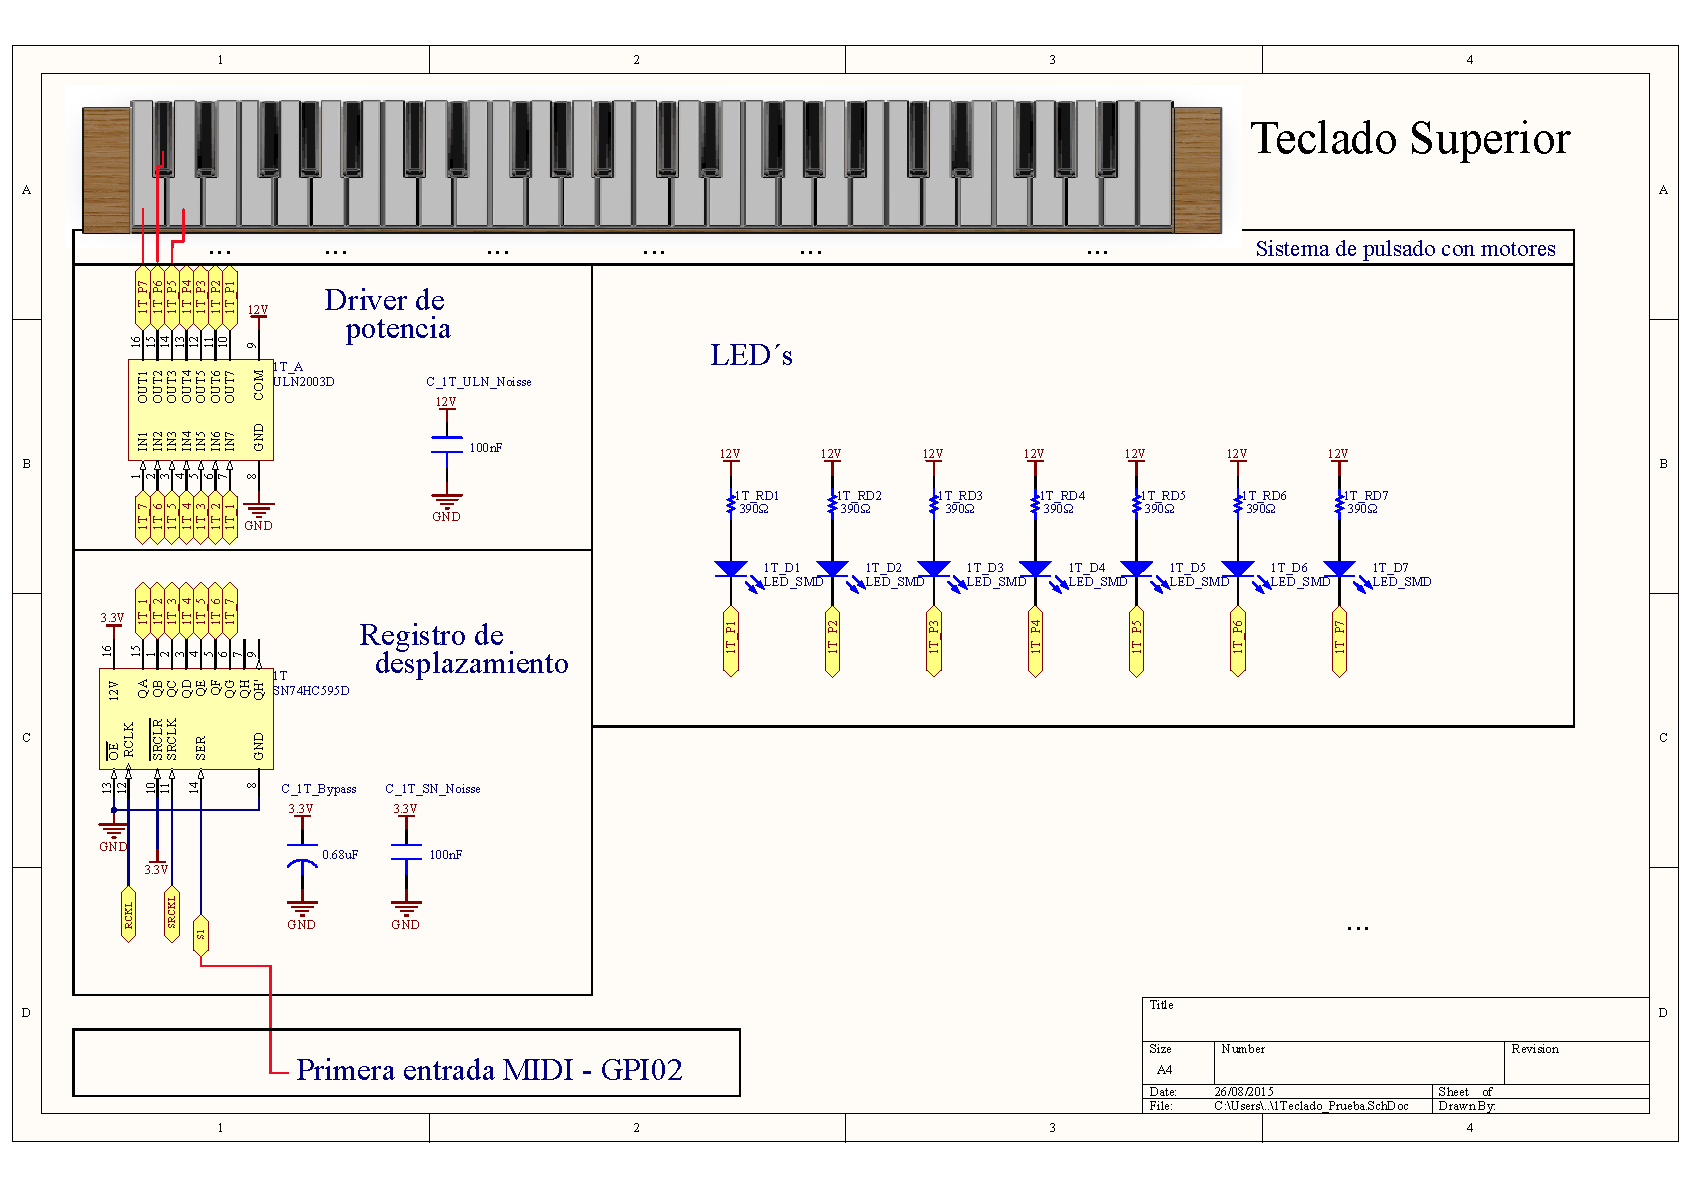
\includegraphics[width=\linewidth*2/3]{capitulo3/pcb_teclado}
		\par\end{centering}
	\smallskip
	\caption{\label{fig:pcb_teclado} Interfaz entre la \acrshort{PCB} y el teclado barroco.}
\end{figure} 

\smallskip

Los dos teclados se comportan de la misma forma, aunque al de abajo le corresponderá un canal diferente.

\subsubsection{Pedalier}

El \textit{pedalier} representa una escala musical, con los pedales bajos similares a las teclas blancas, diatónicas, mientras que los pedales altos emulan a las teclas negras, cromáticas. Por tanto, el esquema de funcionamiento es similar al de los teclados, aunque con menos extensión.

\smallskip

\begin{figure}[H]
	\noindent \begin{centering}
		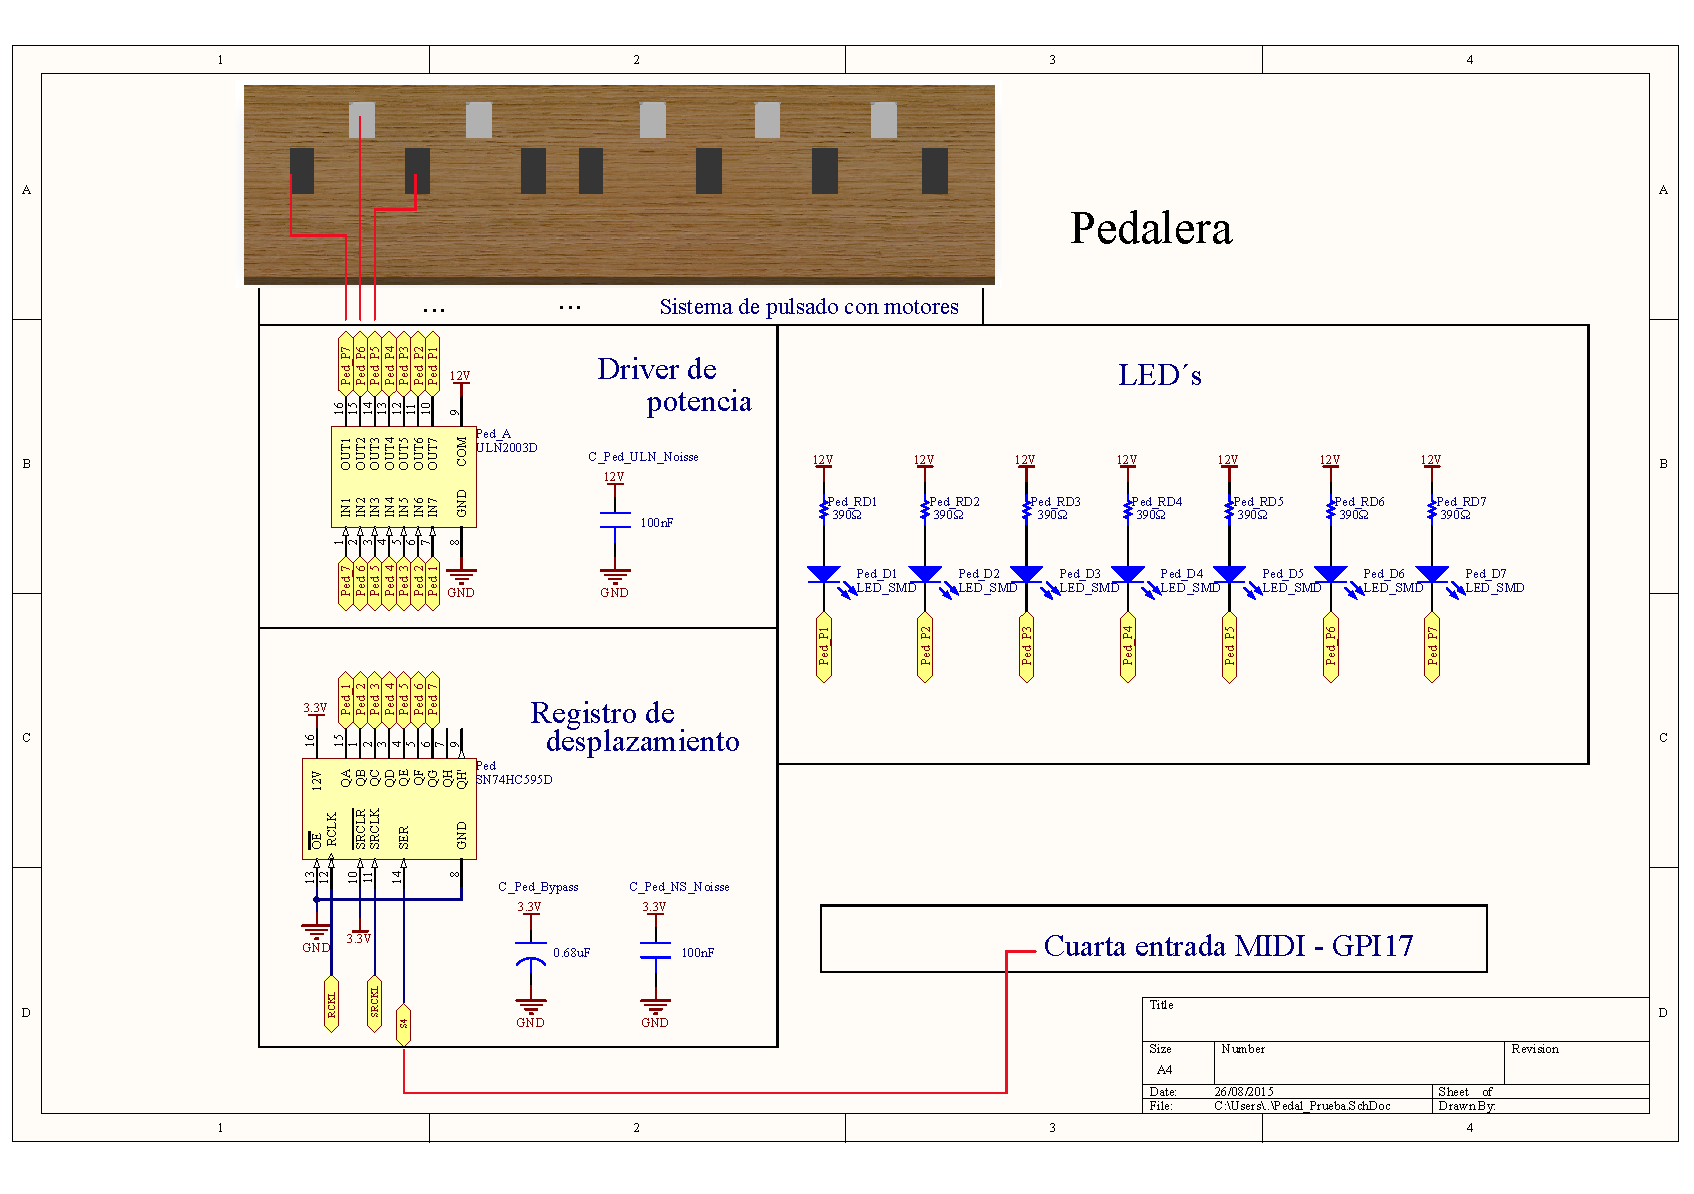
\includegraphics[width=\linewidth*2/3]{capitulo3/pcb_pedalier}
		\par\end{centering}
	\smallskip
	\caption{\label{fig:pcb_pedalier} Interfaz entre la PCB y el pedalier.}
\end{figure} 

\smallskip

\subsubsection{Registros de timbres}

Como podemos ver, los registros no se corresponden con teclas musicales y no tienen el mismo significado. Sin embargo, sí que tienen la misma estructura lógica, al contemplarse dos posiciones: abierto (hacia afuera) y cerrado (hacia dentro).

La mecánica a utilizar será diferente y, probablemente, algo más compleja, pero la interfaz para manejarlos se asemejará a del resto de controles:

\smallskip

\begin{figure}[H]
	\noindent \begin{centering}
		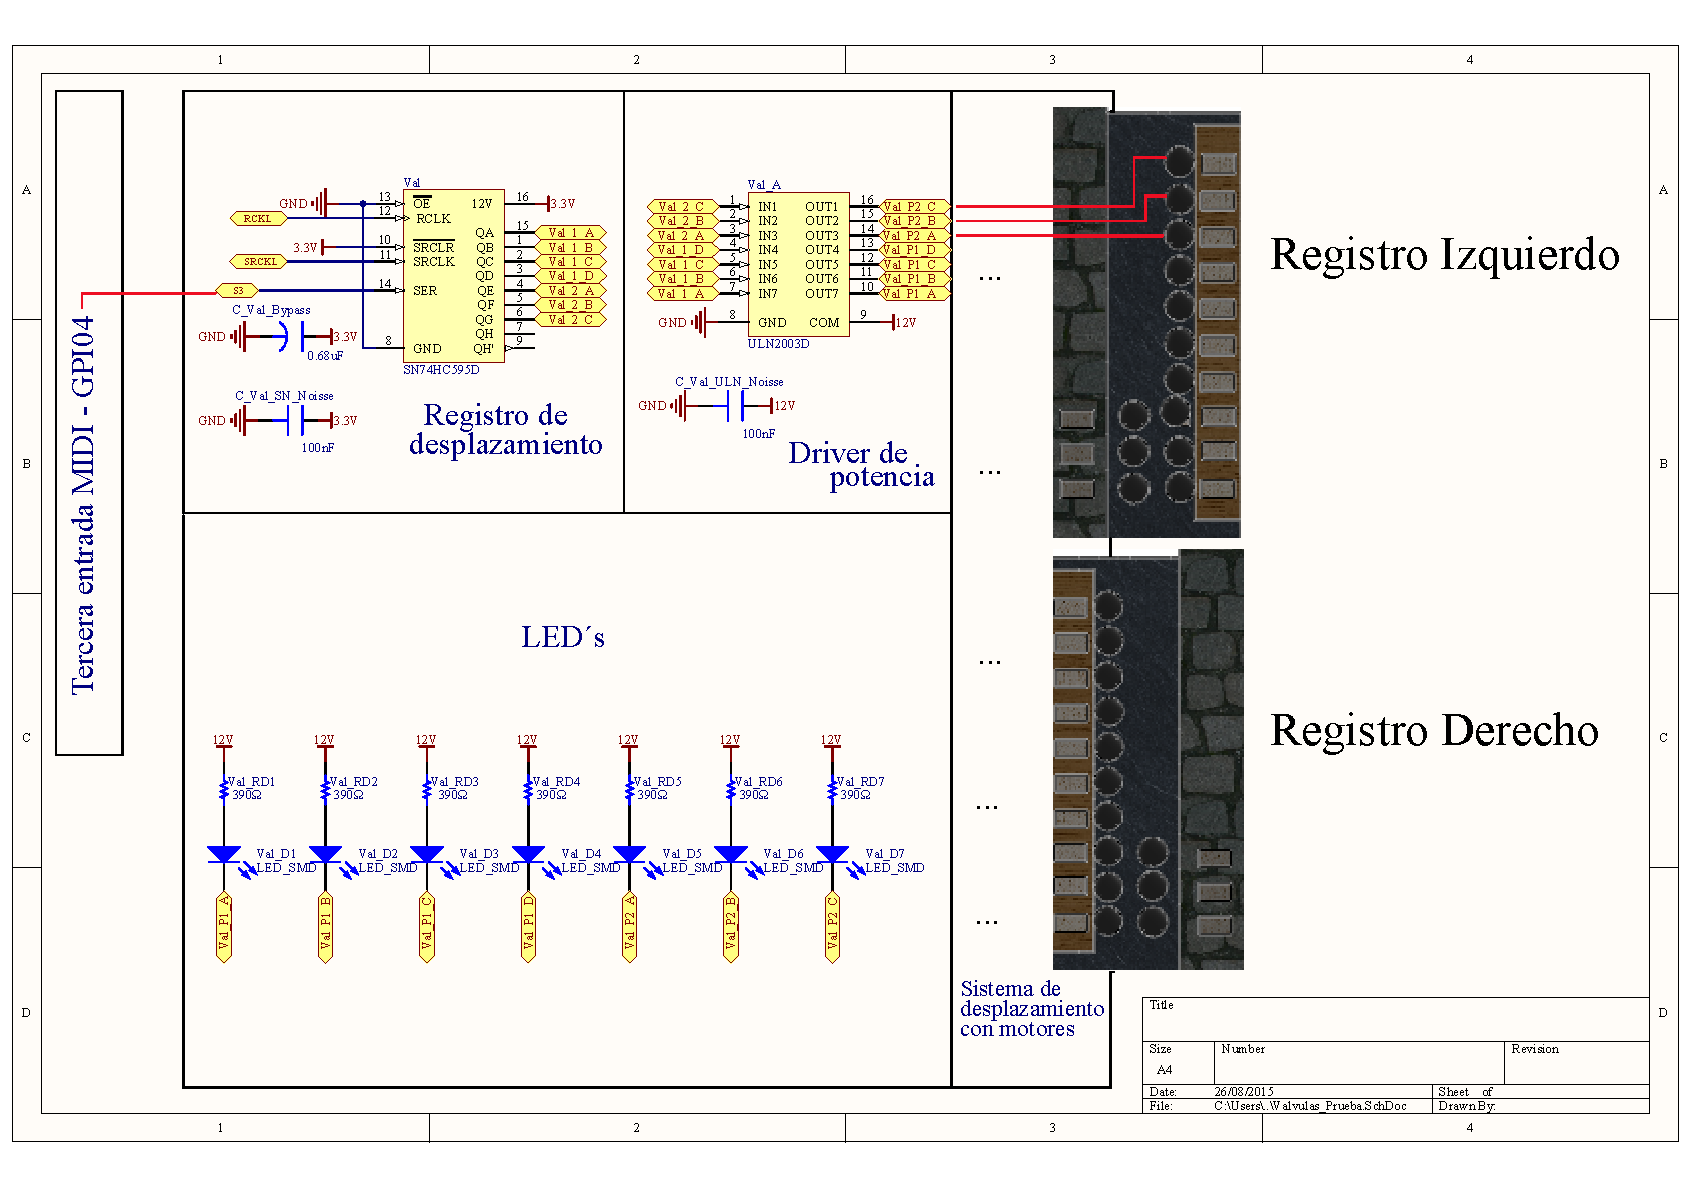
\includegraphics[width=\linewidth*2/3]{capitulo3/pcb_registros}
		\par\end{centering}
	\smallskip
	\caption{\label{fig:pcb_registros} Interfaz entre la PCB y las palancas de registros.}
\end{figure} 

\smallskip

\subsection{Receptor de mando a distancia HIRK-433A}

El receptor de mando a distancia es un detector de radio con decodificador a interfaz RS-232. Nos da la información del número de serie del mando y qué botones han disparado el evento. 

\smallskip

\begin{figure}[H]
	\noindent \begin{centering}
		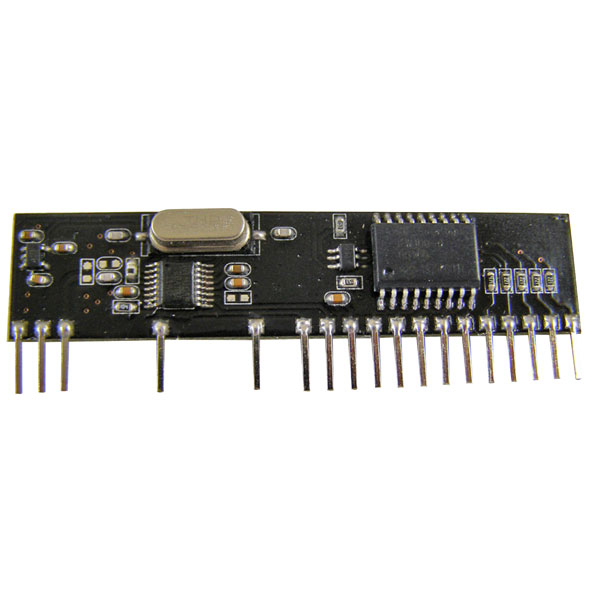
\includegraphics[clip=true,trim=0 200 0 200, width=\linewidth/2]{capitulo3/HIRK-433A}
		\par\end{centering}
	\smallskip
	\caption[Receptor de radio HIRK-433A.]{\label{fig:HIRK-433A} Receptor de radio HIRK-433A. \cite{imagen_decoder}}
\end{figure} 

\smallskip

Es flexible para mandos con distinto número de botones y los indica como un campo de bits basados en la letra A. Si el carácter corresponde a una minúscula, nos avisa de que el mando tiene poca batería. Por ejemplo:

\begin{itemize}
	\item \textbf{A}: Botón 1.
	\item \textbf{B}: Botón 2.
	\item \textbf{C}: Botones 1 y 2.
	\item \textbf{d}: Botón 3 (batería baja).
	\item \textbf{H}: Botón 4.
\end{itemize}

La siguiente tabla muestra los datos de nuestro interés:

\smallskip

\begin{center}
	\begin{tabular}{|l|l|}
		\hline Interfaz & RS-232 \\
		\hline Velocidad & 9600 \textit{baudios} \\ 
		\hline Longitud de trama & 10 \textit{bytes} \\ 
		\hline Sintaxis & <Nº serie (7 \textit{bytes})> <Botón (1 \textit{byte})> <CRLF> \\ 
		\hline 
	\end{tabular}
	\smallskip
	\captionof{table}[Características del receptor de mando.]{\label{tab:info_recv} Características del receptor de mando. \cite{datasheet_decoder}}
\end{center}

\smallskip

\subsection{Pantalla LCD FDCC2004B}

Esta pantalla es un \acrshort{LCD} (\textit{\acrlong{LCD}}) genérico basado en el Hitachi HD44780, considerado un estándar \textit{de facto} para este tipo de dispositivos. Tiene una pequeña memoria para almacenar el estado (no hay que enviar continuamente la información), tiene los caracteres \acrshort{ASCII} predefinidos y tiene capacidad para configurar hasta 8 caracteres especiales.

Esta pieza presenta el siguiente aspecto:

\smallskip

\begin{figure}[H]
	\noindent \begin{centering}
		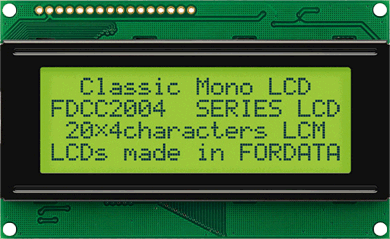
\includegraphics[width=\linewidth/2]{capitulo3/FDCC2004B}
		\par\end{centering}
	\smallskip
	\caption{\label{fig:FDCC2004B} LCD FDCC2004B.}
\end{figure} 

\smallskip

La siguiente tabla muestra sus características principales \cite{datasheet_lcd}:

\smallskip

\begin{center}
	\begin{tabular}{|l|l|}
		\hline Tipo & \acrshort{LCD} retroiluminado \\ 
		\hline Filas & 4 \\ 
		\hline Columnas & 20 \\ 
		\hline Dimensión de celda & 5 x 8 \textit{pixels} \\ 
		\hline Caracteres especiales & 8 \\ 
		\hline 
	\end{tabular}
	\smallskip
	\captionof{table}{\label{tab:info_lcd} Características de la pantalla LCD.}
\end{center} 

\smallskip

\subsection{Codificador rotatorio EC11J}

Un codificador rotatorio es un componente electrónico consistente en un botón giratorio, y emite una señal cuyas características dependen del sentido en que el usuario ha girado el botón. El modelo que vamos a utilizar contiene un botón giratorio y pulsable. \cite{rotary}

\smallskip

\begin{figure}[H]
	\noindent \begin{centering}
		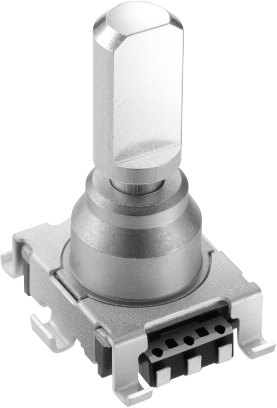
\includegraphics[width=\linewidth/4]{capitulo3/EC11J}
		\par\end{centering}
	\smallskip
	\caption{\label{fig:EC11J} Codificador rotatorio EC11J.}
\end{figure} 

\smallskip

La información nos viene dada por tres canales: uno para el pulsador y dos para la rotación. A medida que rotamos el botón, A y B oscilan produciendo una señal cuadrada que viene desfasada 90\textdegree, como la que aparece en la siguiente imagen:

\smallskip

\begin{figure}[H]
	\noindent \begin{centering}
		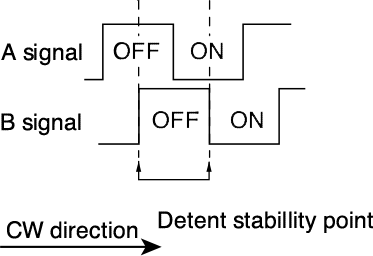
\includegraphics[width=\linewidth/3]{capitulo3/rotary}
		\par\end{centering}
	\smallskip
	\caption{\label{fig:rotary} Código de señales utilizado por el ECJ11.}
\end{figure} 

\smallskip

Los puntos de equilibro ---\textit{detent stability points}--- coinciden con los saltos del canal B, de forma que a la mitad del recorrido de un giro cambiará el canal A. Todo lo que tenemos que hacer entonces es detectar un cambio en A y comparar el valor de A y B: si son iguales, significa que se ha rotado en sentido antihorario; si son distintos, entendemos que se ha girado en sentido horario.

\subsection{Conexión entre la PCB y los periféricos}

\smallskip

\begin{figure}[H]
	\noindent \begin{centering}
		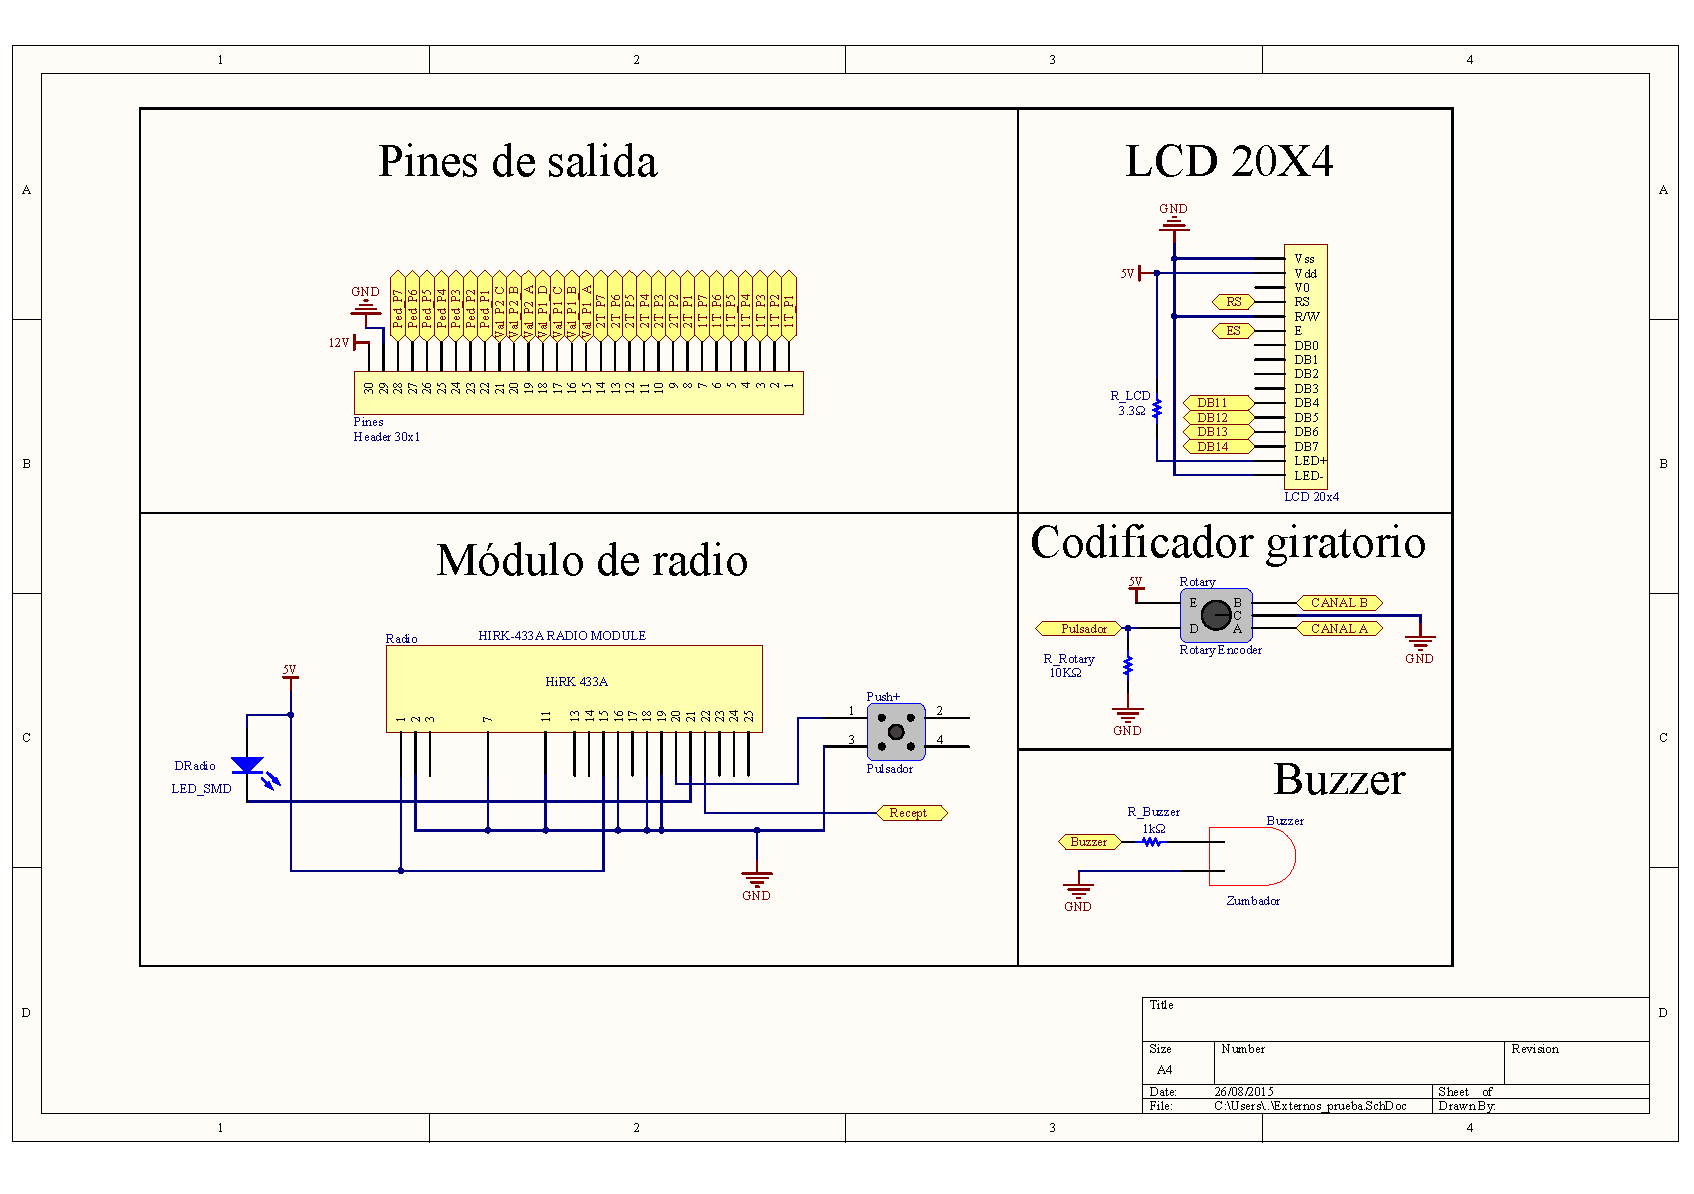
\includegraphics[width=\linewidth*2/3]{capitulo3/pcb_perifericos}
		\par\end{centering}
	\smallskip
	\caption{\label{fig:pcb_perifericos} Interfaz entre la PCB y los periféricos.}
\end{figure} 

\smallskip

\section{SBC Rasberry Pi}

El \textit{Raspberry Pi} es un ordenador de placa única ---\acrshort{PCB} (\textit{\acrlong{SBC}})---, más potente que un microcontrolador y con sistema operativo basado en Linux. Se alimenta por \textit{USB} y se puede controlar con teclado y ratón, o bien desde red mediante \acrshort{SSH}. 

El corazón de este computador es un \acrshort{SOCA} (\textit{\acrlong{SOCA}}), que integra microprocesador, memoria y periféricos principales. El modelo escogido, \textit{B+}, posee numerosos pines de entrada y salida de propósito general (\acrshort{GPIO}), que utilizaremos para interactuar con la \acrshort{PCB} y para ser alimentado por ésta.

\smallskip

\begin{figure}[H]
	\noindent \begin{centering}
		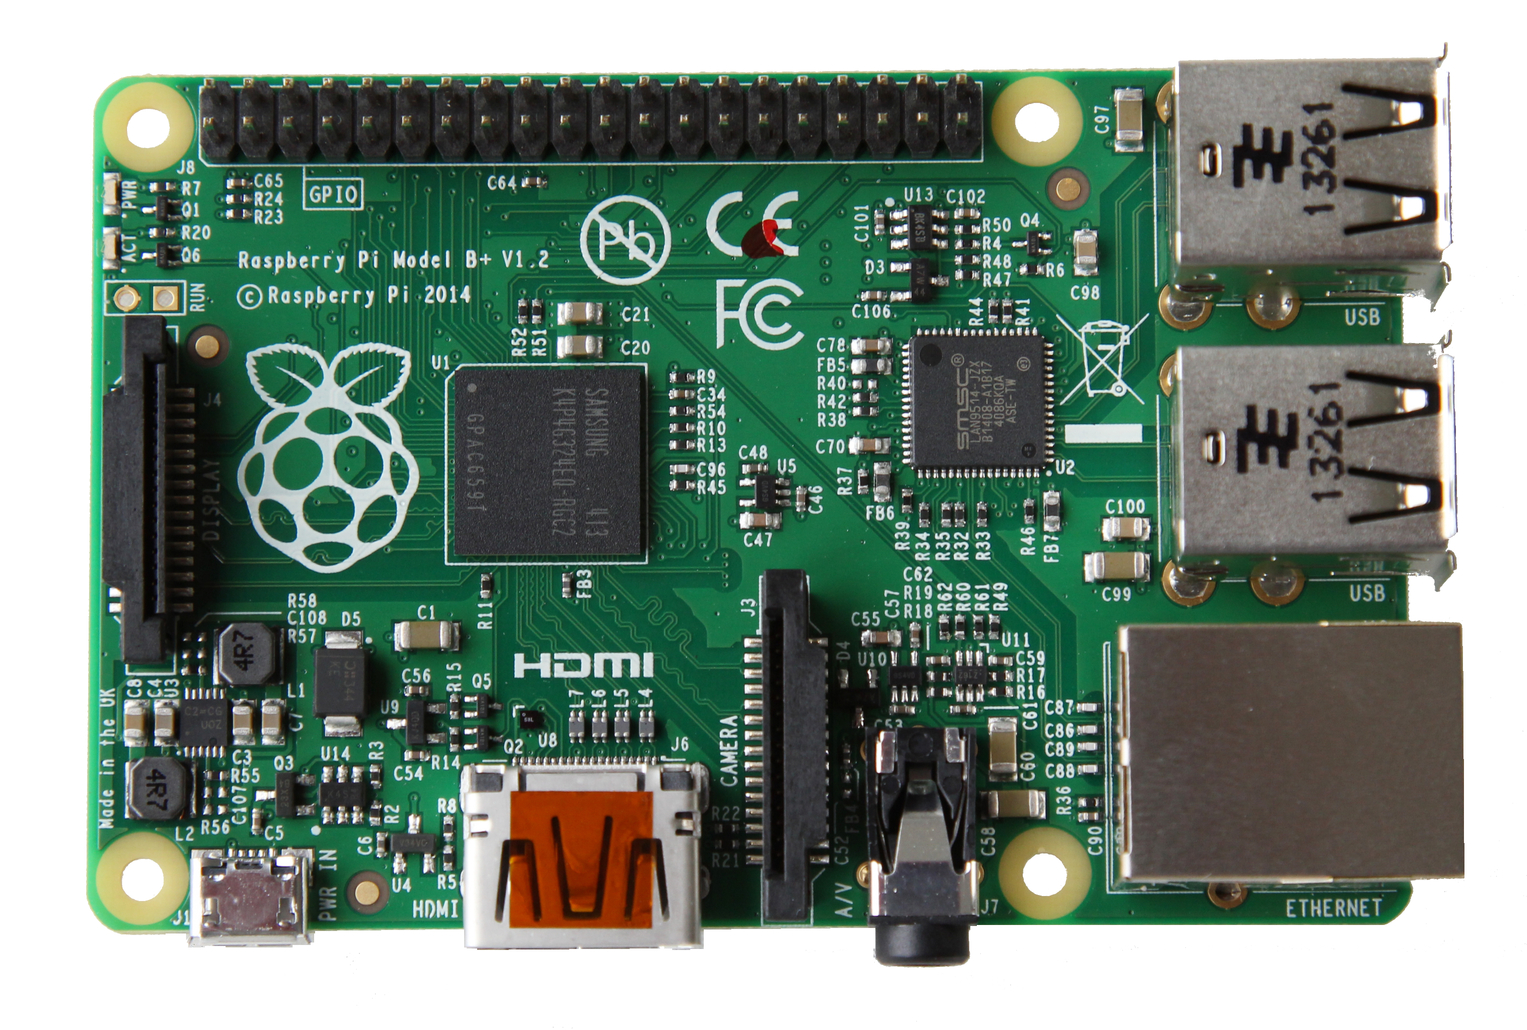
\includegraphics[width=\linewidth/2]{capitulo3/raspberry}
		\par\end{centering}
	\smallskip
	\caption{\label{fig:raspberry} Placa computadora Raspberry Pi.}
\end{figure} 

\smallskip

\subsection{Especificaciones técnicas}

La siguiente tabla ilustra las principales características del \textit{Raspberry Pi} \cite{raspberry}:

\smallskip

\begin{center}
	\begin{tabular}{|l|l|}
		\hline Modelo & Raspberry Pi B+ v1.2 \\
		\hline \acrshort{SOCA} & Broadcom BCM2835 \\
		\hline Procesador &  1176JZF-S @ 700 \textit{MHz} \\
		\hline Repertorio de instrucciones & ARMv6 (\textit{RISC} 32-\textit{bit}) \\
		\hline Memoria & 512 \textit{MB} @ 400 \textit{MHz} \\
		\hline Procesador gráfico & Broadcom VideoCore IV \\ 		
		\hline Almacenamiento & Micro-\acrshort{SD} 8 \textit{GB} \textit{class 10} \\
		\hline Salida de vídeo & \acrshort{HDMI} \\
		\hline Salida de audio & \textit{Jack} 3.5 \textit{mm}, \acrshort{HDMI} \\
		\hline Conectividad USB & 4 x \acrshort{USB} 2.0 \\
		\hline Conectividad de red & \textit{Ethernet} 100 \textit{Mbit/s} \\
		\hline Periféricos & 28xGPIO, \acrshort{UART}, \acrshort{I2C}, \acrshort{SPI} \\ 
		\hline Alimentación & 5V Micro-\acrshort{USB} o \acrshort{GPIO} \\
		\hline Consumo máximo & 1.8 \textit{A} (9 \textit{W}) \\ 
		\hline Sistema operativo & Raspbian (Linux 3.8) \\
		\hline 
	\end{tabular}
	\smallskip
	\captionof{table}{\label{tab:rapberry} Especificaciones del Raspberry Pi.}

\end{center}

\smallskip

\subsection{Pines de E/S}

Como hemos adelantado, la \acrshort{PCB} se conectará al \textit{Raspberry} a través de los conectores \acrshort{GPIO} (\textit{\acrlong{GPIO}}). Todos ellos se utilizarán de forma genérica, excepto el receptor del mando a distancia, que se comunica con la interfaz \textit{RS-232} y debe conectarse al \acrshort{UART} mediante el pin dedicado a tal periférico.

La asignación de pines es la que sigue:

\smallskip

\begin{figure}[H]
	\noindent \begin{centering}
		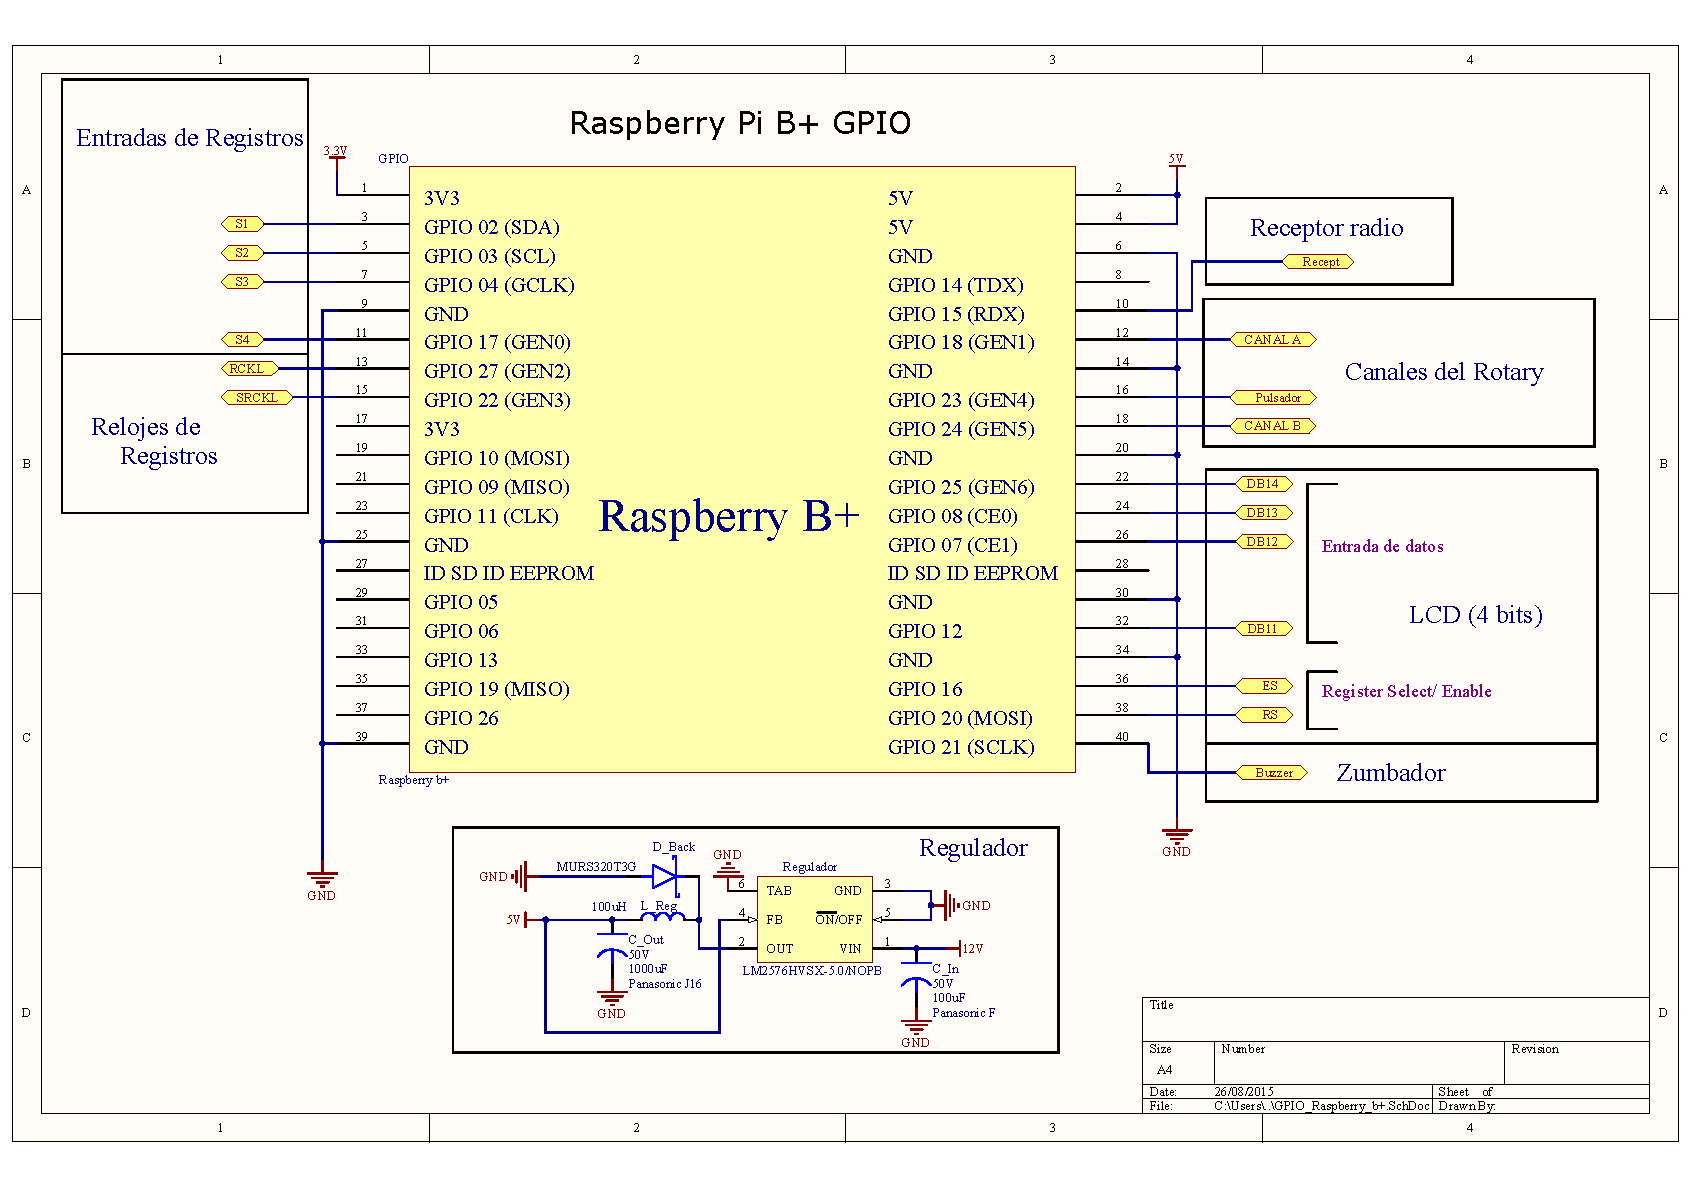
\includegraphics[width=\linewidth*2/3]{capitulo3/pcb_gpio}
		\par\end{centering}
	\smallskip
	\caption{\label{fig:pcb_gpio} Pines de conexión de la PCB con el Raspberry.}
\end{figure} 

\smallskip

\begin{center}
	\begin{tabular}{|l|l|}
		\hline \multicolumn{2}{|c|}{\textbf{Registros de desplazamiento}} \\
		\hline S1 (teclado barroco) & \acrshort{GPIO} 02 \\ 
		\hline S2 (teclado romántico) & \acrshort{GPIO} 03 \\ 
		\hline S3 (registros) & \acrshort{GPIO} 04 \\ 
		\hline S4 (\textit{pedalier}) & \acrshort{GPIO} 17 \\ 
		\hline RCLK (almacenamiento) & \acrshort{GPIO} 27 \\ 
		\hline SRCLK (desplazamiento) & \acrshort{GPIO} 22 \\ 
		\hline \multicolumn{2}{|c|}{\textbf{Receptor de radio}} \\
		\hline O/P-AF (datos) & \acrshort{GPIO} 15 (RDX) \\ 
		\hline \multicolumn{2}{|c|}{\textbf{Pantalla \acrshort{LCD}}} \\
		\hline DB4 (línea 4 del bus) & \acrshort{GPIO} 12 \\ 
		\hline DB5 (línea 5 del bus) & \acrshort{GPIO} 07 \\ 
		\hline DB6 (línea 6 del bus) & \acrshort{GPIO} 08 \\ 
		\hline DB7 (línea 7 del bus) & \acrshort{GPIO} 25 \\
		\hline RS (selección de registro) & \acrshort{GPIO} 20 \\ 
		\hline ES (habilitación de señal) & \acrshort{GPIO} 16 \\ 
		\hline \multicolumn{2}{|c|}{\textbf{Codificador rotatorio}} \\
		\hline Canal A (rotación) & \acrshort{GPIO} 18 \\ 
		\hline Canal B (rotación) & \acrshort{GPIO} 24 \\ 
		\hline Pulsación & \acrshort{GPIO} 23 \\ 
		\hline 
	\end{tabular}
	\smallskip
	\captionof{table}{\label{tab:gpio} Asignaciones de los pines del GPIO.}
\end{center}

\smallskip

\subsection{Sistema operativo}

A pesar de su reducido tamaño, \textit{Raspberry Pi} no es un microcontrolador, sino un microcomputador, con una cantidad notable de recursos \textit{hardware} y potencia de cálculo suficiente para albergar múltiples procesos funcionando concurrentemente. Esto hace necesario el uso de un sistema operativo.

Podemos encontrar varios sistemas operativos compatibles con este computador, pero nosotros vamos a utilizar el sistema oficial, \textit{Raspbian}, una distribución basada en \textit{Debian}, que incorpora el núcleo \textit{GNU/Linux} para la plataforma \textit{ARMv6}.

La introducción de un sistema operativo flexibiliza enormemente la gestión de los recursos \textit{hardware} de un ordenador y garantiza la convivencia equitativa de todos los procesos. Por contra, esto significa que ninguna aplicación podrá utilizar la \textit{CPU} a tiempo completo, ni se garantiza tiempo-real.

El \textit{BCM2835} posee un temporizador de 1 \textit{MHz}. Naturalmente, es inviable ofrecer una granularidad temporal tan fina al planificador; así, éste es llamado cada 10.000 \textit{ticks}, es decir, cada 10 \textit{ms}. Esto garantiza un uso adecuado de los recursos \textit{software} al tiempo que hace imposible realizar comunicaciones síncronas a alta velocidad mediante programación.

Además, la versión utilizada del núcleo Linux es apropiativa ---\textit{preemptive}---, lo que significa que una rutina en modo \textit{kernel} puede bloquearse para dar paso a un servicio de interrupción, incluso que una interrupción puede verse bloqueada por otra de mayor prioridad (interrupciones anidadas).

En conclusión, el uso de un sistema operativo de este tipo, a pesar de ser de gran utilidad, no garantiza sincronismo ni que una espera solicitada sea tan exacta como se pide.

\section{Formato de archivo MIDI}
\label{sec:fmto_midi}

El estándar \acrshort{MIDI} (\acrlong{MIDI}) es una interfaz que permite conectar instrumentos musicales electrónicos y computadoras. Comprende desde un protocolo electrónico hasta un formato de archivos, que se basa en una serie de eventos de control de parámetros musicales. \cite{wiki_midi}

Los datos de entrada a nuestro sistema consisten en archivos \acrshort{MIDI}, tal como se menciona en los requisitos. Este tipo de ficheros se presenta como un conjunto de bloques ---\textit{chunks}--- que contienen los eventos clasificados por pistas. Todos los valores numéricos están en formato \textit{big-endian}, detalle a tener en cuenta, ya que tanto la arquitectura x86 como ARM trabajan en \textit{little-endian}. \cite{midi}

\subsection{Bloque de cabecera}

El bloque de cabecera es siempre el primero, empieza por la firma "MThd" e incluye la siguiente información:

\smallskip

\begin{center}
	\begin{tabular}{|l|l|l|}
		\hline \multicolumn{1}{|c|}{\textbf{Longitud}} & \multicolumn{1}{c|}{\textbf{Descripción}} & \multicolumn{1}{c|}{\textbf{Valor}} \\
		\hline 4 bytes & Firma & "MThd" \\ 
		\hline 4 bytes & Tamaño & 6 \\ 
		\hline 2 bytes & Formato & 0--2 \\ 
		\hline 2 bytes & Número de pistas & 1--65535 \\ 
		\hline 2 bytes & División de tiempo &  \\ 
		\hline 
	\end{tabular}
	\smallskip
	\captionof{table}{\label{tab:midi_header} Contenido de la cabecera MIDI.}
\end{center}

\smallskip

\begin{description}
	\item[Formato] Es la forma en que se organizan las pistas. Puede ser:
	\begin{description}
		\item[0] Una sola pista.
		\item[1] Varias pistas, simultáneas.
		\item[2] Varias pistas, independientes.
	\end{description}
	
	\item[Número de pistas] Indica de cuántas pistas se compone el archivo. Obviamente, si el formato es 0, el valor de este campo será 1.
	
	\item[División de tiempo] Nos indica el significado de cada \textit{tick} de reloj del protocolo como divisiones de una negra (\quarternote). Valores típicos son 96, 120, 180, 192, 240, 360, 384, 480, 640, 720, 768 y 960 \textit{ticks}/\quarternote. Si el \textit{bit} más significativo es 1, el valor indica en su lugar el número de \textit{ticks/fotograma}, habitualmente utilizado en realización de vídeo.
\end{description}

\subsection{Bloque de pista}

Una pista consta de una cabecera y de una lista de eventos, que termina con el meta-evento \textit{fin de pista}.

\smallskip

\begin{center}
	\begin{tabular}{|l|l|l|}
		\hline \multicolumn{1}{|c|}{\textbf{Longitud}} & \multicolumn{1}{c|}{\textbf{Descripción}} & \multicolumn{1}{c|}{\textbf{Valor}} \\
		\hline 4 bytes & Firma & "MTrk" \\ 
		\hline 4 bytes & Tamaño & 0-65535 \\  
		\hline 
	\end{tabular}
	\smallskip
	\captionof{table}{\label{tab:midi_track} Contenido de la cabecera de una pista MIDI.}
\end{center}

\smallskip

\subsection{Eventos MIDI}

Cada evento está formado por los siguientes campos:

\smallskip

\begin{center}
	\begin{tabular}{|l|l|}
		\hline \multicolumn{1}{|c|}{\textbf{Longitud}} & \multicolumn{1}{c|}{\textbf{Descripción}} \\
		\hline Variable & $\Delta$ \\ 
		\hline 1 byte & Tipo de evento y canal \\ 
		\hline 1 byte & Parámetro 1 \\ 
		\hline 1 byte & Parámetro 2 \\ 
		\hline 
	\end{tabular}
	\smallskip
	\captionof{table}{\label{tab:midi_evento} Especificación de un evento MIDI.}
\end{center}

\smallskip

\begin{description}
	\item[$\Delta$] Indica el número de \textit{ticks} que separan al evento actual del precedente.
	\item[Tipo de evento y canal] Los cuatro \textit{bits} más significativos corresponden al tipo de evento. Los otros cuatro marcan el canal \acrshort{MIDI}.
\end{description}

\smallskip

\begin{center}
	\begin{tabular}{|l|l|l|l|}
		\hline \multicolumn{4}{|c|}{\textbf{Tipos de evento}} \\
		\hline \multicolumn{1}{|c|}{\textbf{Valor}} & \multicolumn{1}{c|}{\textbf{Nombre}} & \multicolumn{1}{c|}{\textbf{Parámero 1}} & \multicolumn{1}{c|}{\textbf{Parámetro 2}} \\
		\hline 0x80 & NOTE-OFF & Nota & Velocidad \\
		\hline 0x90 & NOTE-ON & Nota & Velocidad \\
		\hline 0xA0 & NOTE-AFTERTOUCH & Nota & Velocidad \\
		\hline 0xB0 & CONTROLLER & Controlador & Valor \\
		\hline 0xC0 & PROGRAM-CHANGE & Programa &  \\
		\hline 0xD0 & CHANNEL-AFTERTOUCH & Velocidad &  \\
		\hline 0xE0 & PITCH-BEND & \multicolumn{2}{c|}{Valor} \\
		\hline 0xF0 & SYSTEM-EXCLUSIVE & \multicolumn{2}{c|}{} \\
		\hline 0xFF & Meta-evento & \multicolumn{2}{c|}{} \\
		\hline 
	\end{tabular}
	\smallskip
	\captionof{table}{\label{tab:midi_eventos} Eventos MIDI.}
\end{center}

\smallskip

\subsubsection{Meta-eventos}

Los metaeventos son mensajes de control que extienden la semántica de los eventos normales. Tienen la siguiente estructura:

\smallskip

\begin{center}
	\begin{tabular}{|l|l|}
		\hline \multicolumn{1}{|c|}{\textbf{Longitud}} & \multicolumn{1}{c|}{\textbf{Descripción}} \\
		\hline Variable & $\Delta$ \\ 
		\hline 1 byte & 0xFF \\
		\hline 1 byte & Tipo de metaevento \\
		\hline Variable & Longitud del argumento \\ 
		\hline (Longitud) & Valor del argumento \\ 
		\hline
	\end{tabular}
	\smallskip
	\captionof{table}{\label{tab:midi_mevaevento} Especificación de un meta-evento MIDI.}
\end{center}

\smallskip

Los tipos de meta-evento estándar son los siguientes:

\smallskip

\begin{center}
	\begin{tabular}{|l|l|}
		\hline \multicolumn{2}{|c|}{\textbf{Tipos de meta-evento}} \\
		\hline \multicolumn{1}{|c|}{\textbf{Valor}} & \multicolumn{1}{c|}{\textbf{Nombre}} \\
		\hline 0x00 & Número de secuencia \\
		\hline 0x01 & Texto \\
		\hline 0x02 & Noticia de \textit{copyright} \\
		\hline 0x03 & Nombre de la secuencia \\
		\hline 0x04 & Nombre del instrumento \\
		\hline 0x05 & Letra de la canción \\
		\hline 0x06 & Marca \\
		\hline 0x07 & Punto de corte \\
		\hline 0x08 & Nombre del programa \\
		\hline 0x09 & Nombre del dispositivo \\
		\hline 0x20 & Canal por defecto (obsoleto) \\
		\hline 0x21 & Puerto por defecto (obsoleto) \\
		\hline 0x2F & Fin de pista \\
		\hline 0x51 & \textit{Tempo} ($\mu s/\quarternote$) \\
		\hline 0x54 & Desplazamiento temporal \\
		\hline 0x58 & Indicación de compás \\
		\hline 0x59 & Indicación de tonalidad \\
		\hline 0x7F & Reservado para el secuenciador \\
		\hline 
	\end{tabular}
	\smallskip
	\captionof{table}{\label{tab:midi_metaeventos} Meta-eventos MIDI.}
\end{center}

\smallskip

\subsubsection{Notas}

Las notas en \acrshort{MIDI} se indican numéricamente, en base 0, asignando valores a las notas cromáticas a partir de \textit{Do -1}. Por ejemplo, al \textit{Do central (Do 4)} le corresponde el valor 60.

\section{Esquema de interconexión general}

Todos los elementos que hemos descrito conformarán la parte \textit{hardware} del sistema y establecerán una conexión cuyos extremos son el computador \textit{Raspberry Pi} y los mecanismos que interactuarán con la consola del órgano.

A continuación presentamos un diagrama que describe a \textit{grosso modo} la conexión lógica entre todos los elementos \textit{hardware}:

\smallskip

\begin{figure}[H]
	\noindent \begin{centering}
		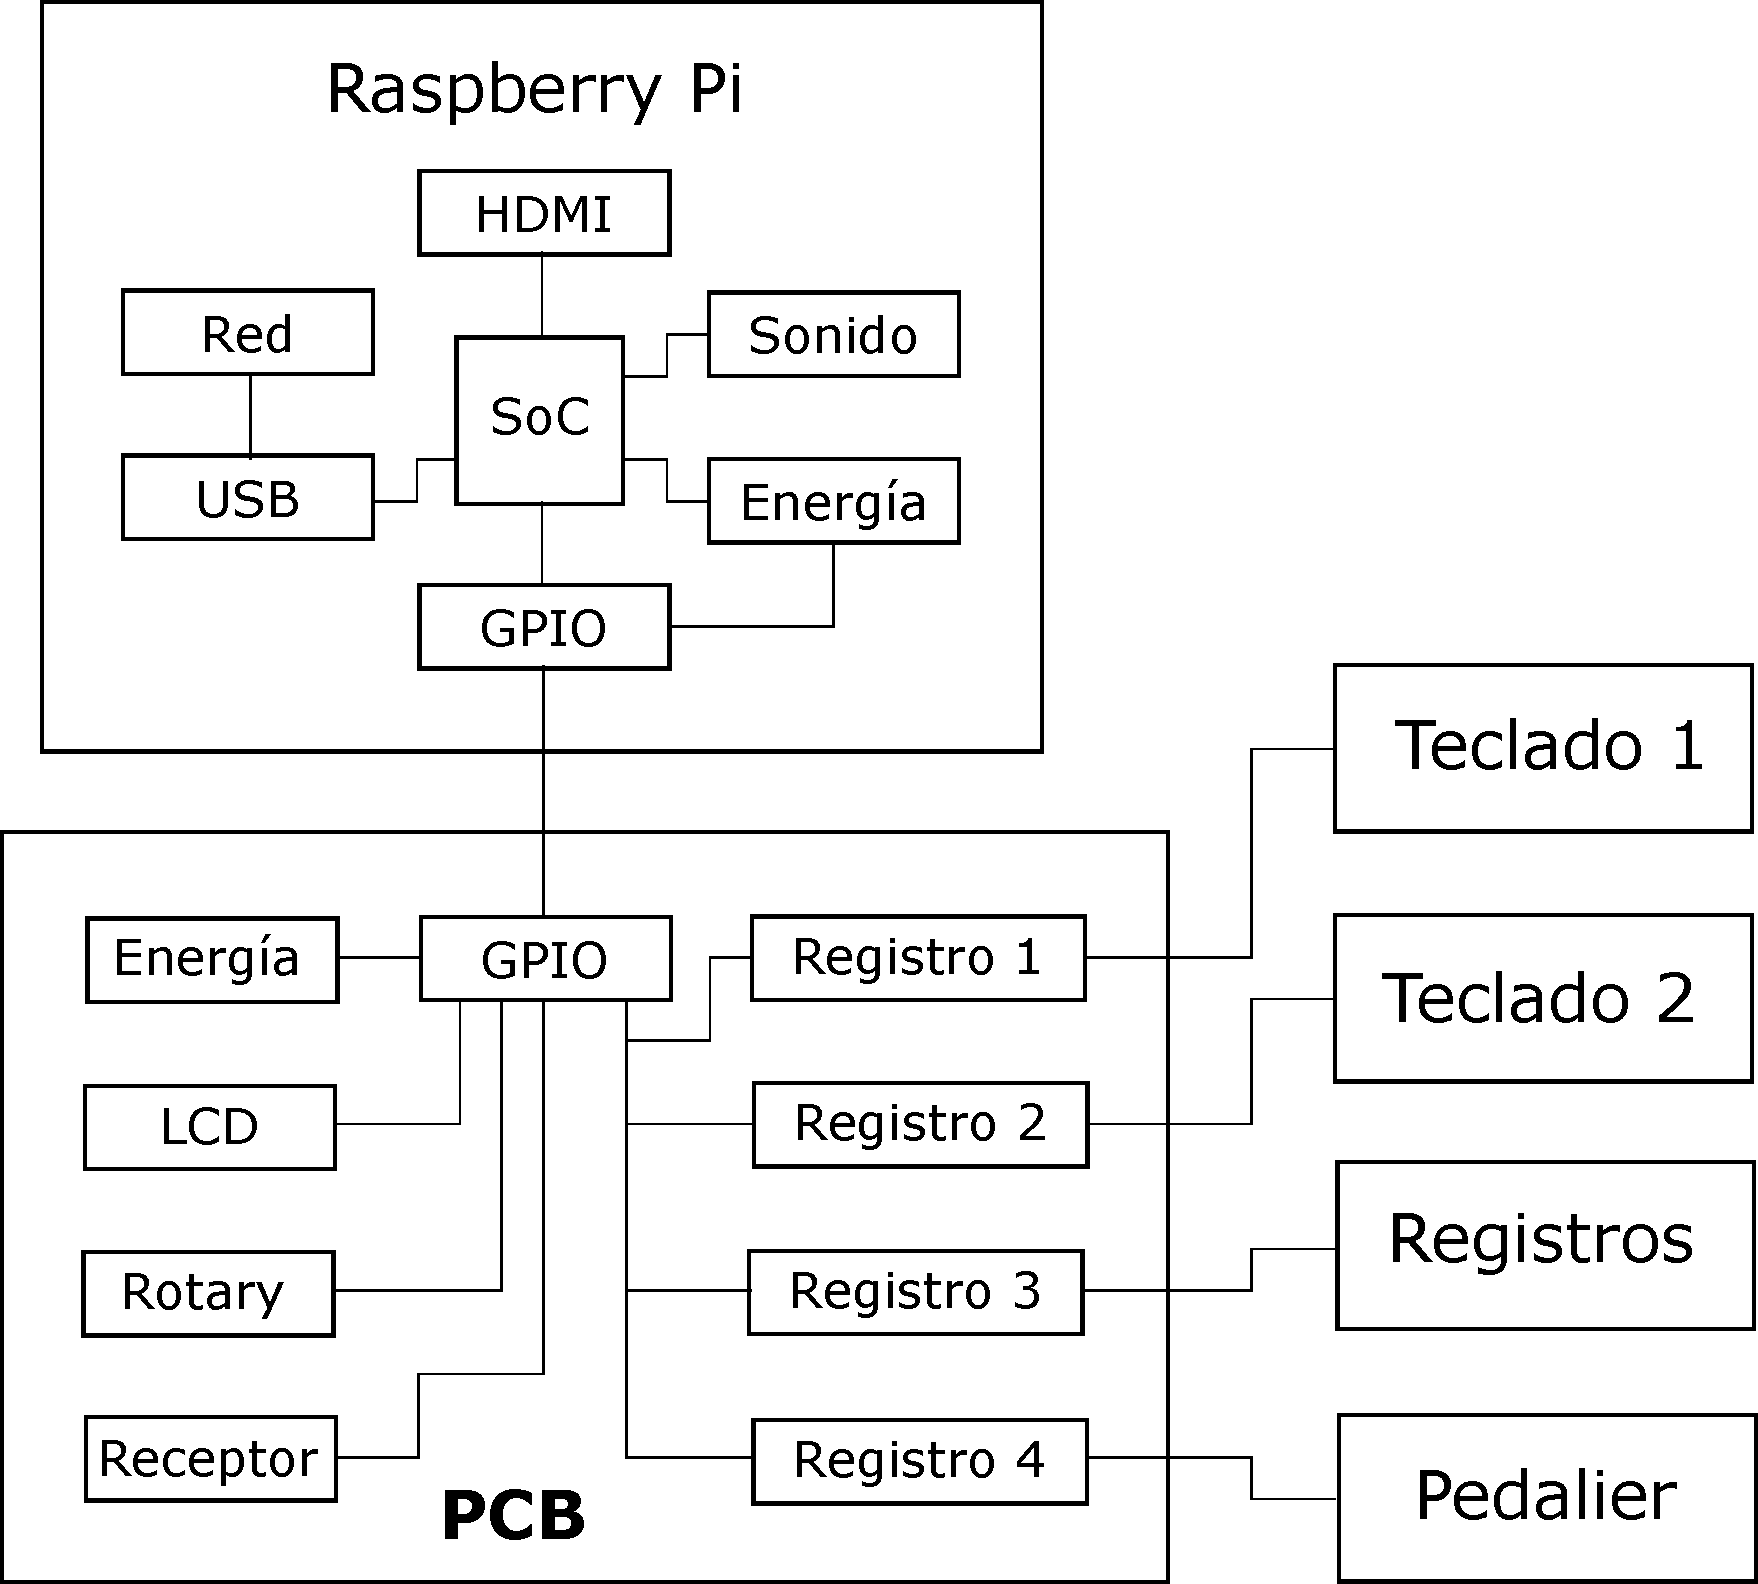
\includegraphics[width=\linewidth*2/3]{capitulo3/hardware}
		\par\end{centering}
	\smallskip
	\caption{\label{fig:hardware} Conexión lógica entre los elementos hardware.}
\end{figure} 

\smallskip

La \acrshort{PCB} incorpora una fuente de alimentación para el \textit{Raspberry}, que está conectada mediante la interfaz \acrshort{GPIO}. Todas las conexiones harán funcionar los mecanismos del órgano, pasando por los registros de desplazamiento, que retendrán el estado.

El resto de periféricos nos serán de utilidad para desarrollar un sistema que cumplirá todos los requisitos contemplados en el capítulo \ref{cap:capitulo_2}.

\clearpage{\cleardoublepage}
\clearpage{\pagestyle{empty}\cleardoublepage}